\documentclass[12pt]{article}
\usepackage[a4paper, left=2.5cm, right=2.5cm, top=2.5cm, bottom=1.25cm]{geometry}
\usepackage{newtxtext}
\usepackage{graphicx}
\usepackage{enumitem}
\usepackage{cite}   % improves citation formatting
\usepackage{url}    % handles URLs safely
\usepackage{setspace}
\usepackage{array}
\usepackage{float}
\usepackage{graphicx}


\begin{document}
\begin{center}

% Report Type
{\fontsize{16pt}{20pt}\selectfont
\textbf{A MIDTERM PROGRESS REPORT}}\\[1cm]
{\fontsize{16pt}{20pt}\selectfont
\textbf{On}}\\[1cm]

% Project Title
{\fontsize{24pt}{28pt}\selectfont
\textbf{BLOCKCHAIN SECURE VAULT}}\\[1cm]

% Submission Statement
{\fontsize{12pt}{14pt}\selectfont
\textbf{Submitted in partial fulfillment of the requirements for the award of}}\\[0.4cm]

{\fontsize{12pt}{14pt}\selectfont
\textbf{the degree of}}\\[0.5cm]

% Degree
{\fontsize{14pt}{18pt}\selectfont
\textbf{BACHELOR OF TECHNOLOGY}}\\[0.7cm]

% Branch
{\fontsize{14pt}{18pt}\selectfont
Computer Science and Engineering}\\[1cm]

% Submitted By
{\fontsize{12pt}{14pt}\selectfont
SUBMITTED BY}\\[0.8cm]

% Student Names and University Roll Numbers
\begin{tabular}{c@{\hspace{1cm}}c@{\hspace{1cm}}c}
{\fontsize{14pt}{16pt}\selectfont EKAMPREET SINGH} &
{\fontsize{14pt}{16pt}\selectfont GAURAV PRASHAR} &
{\fontsize{14pt}{16pt}\selectfont GAURAV SHARMA} \\[0.3cm]

{\fontsize{12pt}{14pt}\selectfont 2302515} &
{\fontsize{12pt}{14pt}\selectfont 2302518} &
{\fontsize{12pt}{14pt}\selectfont 2302519}
\end{tabular}\\[1.2cm]

% Under the Guidance
{\fontsize{12pt}{14pt}\selectfont
UNDER THE GUIDANCE OF}\\[0.5cm]

{\fontsize{14pt}{16pt}\selectfont
ASST PROF. MEETALI}\\[1.2cm]

% Month and Year
{\fontsize{12pt}{14pt}\selectfont
OCTOBER 2026}\\[1.2cm]

% GNDEC Logo

\includegraphics[width=4cm]{gne_logo.png}\\[1.2cm]

% Department
{\fontsize{12pt}{14pt}\selectfont
\textbf{Department of Computer Science and Engineering}}\\[0.5cm]

% College Name
{\fontsize{16pt}{20pt}\selectfont
\textbf{GURU NANAK DEV ENGINEERING COLLEGE,}}\\[0.5cm]

{\fontsize{16pt}{20pt}\selectfont
\textbf{LUDHIANA}}

\end{center}


\newpage
\tableofcontents
\newpage
\listoftables
\addcontentsline{toc}{section}{List of Tables}

\clearpage

\listoffigures
\addcontentsline{toc}{section}{List of Figures}

\newpage
\section{Introduction}

\subsection{Brief introduction about the project to be developed}

This project is an extended and enhanced version of the previously developed Blockchain Secure Vault, continued as a major project through the development of a dedicated mobile application for secure document management. The existing system provides encrypted document storage, decentralized storage, and blockchain-based integrity verification. The major project focuses on extending this foundation with a convenient mobile interface while improving document organization, accessibility, and access control. The proposed system combines end-to-end encryption, decentralized storage, blockchain-based verification, and application-level security to provide a secure environment for managing sensitive digital documents \cite{stallings2017}.

The mobile application will enable authorized users to securely access, organize, search, share, and manage their encrypted documents. It will introduce a file-manager interface with folders and subfolders, document search, role-based access control, and temporary access permissions. Users will also be able to view supported documents within the application and access downloaded documents through controlled in-app workflows. Temporary access can be granted for a predefined duration and automatically becomes invalid after expiration, while role-based permissions ensure that users can perform only authorized operations. The mobile application will communicate with the existing backend and blockchain infrastructure, allowing the security mechanisms developed during the minor project to be utilized and extended in the major project.

The project aims to provide a practical and secure mobile solution for document management while maintaining confidentiality, integrity, and controlled accessibility. By combining blockchain, cryptography, decentralized storage, secure backend services, and mobile application development, the project demonstrates the practical application of these technologies in a comprehensive secure document management system.

\subsection{Technology Used}
\begin{itemize}
\item \textbf{Mobile Application:} React Native for developing the cross-platform mobile application
\item \textbf{Backend:} Node.js and Express for REST APIs, authentication, access control, and document management
\item \textbf{Database:} MongoDB for user accounts, document metadata, folders, permissions, and access records
\item \textbf{Blockchain:} Solidity smart contracts with Hardhat and Ethers.js for on-chain integrity verification
\item \textbf{Storage:} IPFS with Pinata for decentralized storage of encrypted documents
\item \textbf{Cryptography:} AES-256 for document encryption and SHA-256 for integrity hashing \cite{nist197}
\item \textbf{Document Processing:} PDF.js, Mammoth.js, and suitable mobile document-rendering libraries for secure in-app document viewing
\end{itemize}

\subsection{Field of Project}
\begin{itemize}
\item Information and Cyber Security
\item Blockchain and Decentralized Storage
\item Secure Mobile Application Development
\item Secure Document and File Management
\item Access Control and Privacy
\end{itemize}

\subsection{Special Technical Terms}
\begin{itemize}
\item \textbf{End-to-End Encryption (E2EE):} Documents are encrypted before storage and decrypted only when accessed by an authorized user.
\item \textbf{Content Hash:} A cryptographic fingerprint used to identify a document and detect unauthorized modification.
\item \textbf{On-chain Verification:} Verification of document integrity by comparing its computed hash with the corresponding blockchain record.
\item \textbf{Role-Based Access Control (RBAC):} A security mechanism in which document permissions are assigned according to the user's role and authorized operations.
\item \textbf{Temporary Access:} Time-limited permission that automatically expires after a predefined duration.
\item \textbf{Immutable Ledger:} A tamper-resistant blockchain record used to maintain trustworthy document integrity information.
\item \textbf{In-App Document Viewing:} A controlled mechanism for viewing supported documents within the mobile application without unnecessarily exposing decrypted files to external applications.
\end{itemize}


\subsection{Objectives}

\begin{enumerate}
    \item To develop a secure mobile application for streamlined document management and organization.
    
    \item To establish role-based access control for secure document sharing.
    
   \item To enable efficient document search and folder-based organization with in-app viewing through secure access mechanisms
\end{enumerate}


\newpage
\section{System Requirements}

The Major Project extends the existing Secure Document Vault by introducing a mobile application for secure document management and controlled access. The system requirements therefore focus primarily on the hardware and software required to develop and operate the mobile application and its supporting services.

\subsection{Software Requirements}

The following software technologies and development tools are required for the development and execution of the extended system:

\begin{table}[h]
\centering
\caption{Software Requirements}
\label{tab:software_requirements}
\renewcommand{\arraystretch}{1.3}
\begin{tabular}{|p{4cm}|p{9cm}|}
\hline
\textbf{Software / Technology} & \textbf{Purpose} \\ \hline

\textbf{React Native} & Development of the cross-platform mobile application \\ \hline

\textbf{Expo} & Development, testing, and execution of the React Native mobile application \\ \hline

\textbf{Expo Router} & Management of application navigation and screen routing \\ \hline

\textbf{TypeScript} & Type-safe development of the mobile application \\ \hline

\textbf{NativeWind} & Styling and responsive user-interface development \\ \hline

\textbf{Axios} & Communication between the mobile application and backend REST APIs \\ \hline

\textbf{Expo SecureStore} & Secure storage of authentication tokens and sensitive session information on the mobile device \\ \hline

\textbf{Node.js} & Runtime environment for the existing backend services \\ \hline

\textbf{Express.js} & Backend REST API framework used by the mobile application \\ \hline

\textbf{MongoDB} & Storage of document-related metadata, user information, sharing information, and access-related data \\ \hline

\textbf{Git / GitHub} & Source-code management and version control \\ \hline

\textbf{Visual Studio Code} & Primary development environment for source-code development and debugging \\ \hline

\end{tabular}
\end{table}

The mobile application communicates with the existing backend through REST APIs rather than implementing a separate backend. This allows the mobile application to reuse the existing document-management and authorization services.

The system provides authentication and authorization mechanisms that support controlled access to documents. These mechanisms include existing and modified JWT-based authentication and role-based authorization functionalities, adapted to meet the requirements of the enhanced system.

\subsection{Hardware Requirements}

The following hardware is required for development, testing, and operation of the system:

\begin{table}[h]
\centering
\caption{Hardware Requirements}
\label{tab:hardware_requirements}
\renewcommand{\arraystretch}{1.3}
\begin{tabular}{|p{4cm}|p{9cm}|}
\hline
\textbf{Hardware} & \textbf{Minimum / Recommended Requirement} \\ \hline

\textbf{Development Computer} & Intel Core i5 or equivalent processor \\ \hline

\textbf{RAM} & Minimum 8 GB; 16 GB recommended for smoother development \\ \hline

\textbf{Storage} & Minimum 20 GB of available storage for development tools, dependencies, Android SDK, and project files \\ \hline

\textbf{Internet Connection} & Required for package installation, backend communication, API access, and development services \\ \hline

\textbf{Android Device / Emulator} & Android device or emulator for testing the mobile application \\ \hline

\textbf{Mobile Storage} & Sufficient storage for application installation and temporary document handling \\ \hline

\end{tabular}
\end{table}

\subsection{Mobile Application Requirements}

The mobile application requires an Android-compatible environment for installation and execution. During development, the application can be tested using either a physical Android device or an Android emulator.

The application requires network connectivity to communicate with the existing backend services. Authentication information is securely stored on the mobile device, while document-related operations are performed through the backend APIs.

\subsection{Requirements Related to Project Objectives}

The system requirements directly support the three major objectives of the project:

\begin{enumerate}

    \item \textbf{Secure Mobile Document Management}

    The React Native and Expo environment provides the platform for developing the mobile application through which users can manage their documents.

    \item \textbf{Role-Based Access Control}

    The existing authentication and authorization infrastructure provides role and organization-level access checks, which are used to control document-related operations.

    \item \textbf{Document Search, Organization and Controlled Viewing}

    The backend provides document retrieval, sharing, downloading, and viewing operations that can be accessed by the mobile application. File and folder organization is being extended as part of the Major Project.

\end{enumerate}
The requirements described above are sufficient to support the implementation and testing of the major-project objectives without unnecessarily repeating the complete requirements of the original Minor Project.

\newpage

\section{Software Requirement Analysis}

\subsection{Problem Definition}

The existing Secure Document Vault provides a secure foundation for storing, accessing, sharing, and verifying digital documents. However, the earlier system primarily focused on the underlying secure document infrastructure and web-based access. There is a need to extend this functionality to a mobile environment so that users can manage their documents more conveniently while maintaining controlled access.

The Major Project addresses this requirement by extending the existing system with a mobile application focused on secure document management, controlled sharing, document retrieval, and organization. The mobile application communicates with the existing backend services and provides a mobile-oriented interface for the required document operations. The repository contains both an Expo/React Native mobile application and a shared Node.js/Express backend.

The main problems addressed by the Major Project are:

\begin{itemize}
    \item Difficulty in managing and accessing documents conveniently through a mobile platform.
    
    \item Requirement for controlled document sharing based on user roles and permissions.
    
    \item Difficulty in efficiently locating and organizing documents as the number of stored documents increases.
    
    \item Requirement for controlled access to documents instead of unrestricted viewing or sharing.
    
    \item Need to extend the existing Secure Document Vault without duplicating the complete backend system.
\end{itemize}

Therefore, the Major Project concentrates on providing a mobile interface and supporting functionality for secure document management, role-based access, document search, folder-based organization, and controlled document viewing.


% ---------------------------------------------------------
\subsection{Existing System}

The existing system was developed as the Minor Project and provides the foundation for the current Major Project. It includes secure document management functionality together with authentication, document storage, sharing and verification.

For the Major Project, these existing services are reused wherever possible. The mobile application communicates with the existing backend through APIs instead of creating an independent backend. This reduces duplication and allows the new mobile functionality to work with the existing document-management infrastructure.


% ---------------------------------------------------------
\subsection{Proposed System}

The proposed system is an extension of the Secure Document Vault that introduces and enhances mobile-based document management. The system provides users with a mobile interface through which they can manage documents while access to documents is controlled according to authorization rules.

The proposed system focuses on three major areas:


% ---------------------------------------------------------
\subsubsection{Secure Mobile Document Management}

A mobile application is developed using React Native and Expo to provide users with a convenient interface for document-related operations. The application communicates with the existing backend through REST APIs.

The mobile application provides the interface required for managing documents and accessing the functionality of the Secure Document Vault from a mobile device. The repository identifies the mobile application as an Expo/React Native client located under the mobile application directory.


% ---------------------------------------------------------
\subsubsection{Role-Based Access Control}

The proposed system provides controlled access to documents according to user roles and organizational permissions. The authorization layer validates authenticated users and applies organization or membership-based access checks before allowing protected operations.

The existing implementation includes JWT-based authentication. Role-based access control is identified as an implemented functional requirement in the project analysis.

This mechanism forms the basis for secure document sharing by ensuring that users can perform document operations only when they have the required permissions.


% ---------------------------------------------------------
\subsubsection{Document Search, Organization and Controlled Viewing}

The system provides document retrieval functionality so that users can locate and access documents associated with their authorized user or organization context. Document download and viewing functionality is also present in the existing system.

The Major Project further focuses on improving document organization through folder-based management and providing controlled in-app access to documents. File/folder management is currently not implemented, making it one of the areas to be further developed during the project.


% ---------------------------------------------------------
\subsection{Functional Requirements}

The functional requirements relevant to the Major Project are as follows:
\begin{table}[H]
\centering
\caption{Functional Requirements of the Major Project}
\label{tab:functional_requirements}
\renewcommand{\arraystretch}{1.35}
\begin{tabular}{|c|p{4.0cm}|p{8.0cm}|}
\hline
\textbf{ID} &
\textbf{Functional Requirement} &
\textbf{Description} \\ \hline

FR-01 &
Mobile Application &
Provide a mobile interface for secure document-management operations. \\ \hline

FR-02 &
User Authentication &
Allow authenticated users to access protected mobile functionality. \\ \hline

FR-03 &
Document Management &
Allow users to access and manage documents through the mobile application. \\ \hline

FR-04 &
Document Search &
Allow users to retrieve documents according to their authorized user or organization context. \\ \hline

FR-05 &
Document Sharing &
Allow documents to be shared with authorized users. \\ \hline

FR-06 &
Role-Based Access Control &
Restrict document operations according to user roles and permissions. \\ \hline

FR-07 &
Controlled Access &
Ensure protected document operations are available only to authorized users. \\ \hline

FR-08 &
Document Viewing &
Allow authorized users to view documents through the application. \\ \hline

FR-09 &
Folder/File Organization &
Organize documents using file/folder-based management. \\ \hline

FR-10 &
Mobile-to-Backend Communication &
Communicate with the existing backend through REST APIs. \\ \hline

\end{tabular}
\end{table}

The project analysis specifically identifies document search, document download, document viewing, role-based access control, temporary access, and the mobile application among the implemented requirements, while file/folder management is not implemented.


% ---------------------------------------------------------
\subsection{Modules of the Proposed System}

To keep the Major Project focused on its defined objectives, the relevant modules are organized as follows.


% ---------------------------------------------------------
\subsubsection{Module 1: Mobile Application Module}

\textbf{Purpose:}

Provide a mobile interface for accessing and managing documents.

\textbf{Main responsibilities:}

\begin{itemize}
    \item Provide mobile screens for document-related operations.
    \item Communicate with backend APIs.
    \item Manage authenticated user sessions.
    \item Display documents and their relevant information.
    \item Provide user interaction for search, organization, sharing, and viewing.
\end{itemize}

\textbf{Technology:} React Native, Expo, Expo Router, TypeScript.

\textbf{Status:} Implemented.


% ---------------------------------------------------------
\subsubsection{Module 2: Document Management Module}

\textbf{Purpose:}

Manage the user's documents and provide access to document-related operations.

\textbf{Main responsibilities:}

\begin{itemize}
    \item Retrieve documents.
    \item Display document information.
    \item Support document access and download.
    \item Support document viewing.
    \item Apply access restrictions before protected operations.
\end{itemize}

The repository identifies document management as responsible for uploading, listing, sharing, downloading, and verifying documents.


% ---------------------------------------------------------
\subsubsection{Module 3: Role-Based Access Control Module}

\textbf{Purpose:}

Control document access according to the authenticated user's permissions and organizational role.

\textbf{Main responsibilities:}

\begin{itemize}
    \item Validate the user's authentication token.
    \item Check authorization before protected operations.
    \item Apply organization-level access rules.
    \item Restrict operations to authorized users or members.
\end{itemize}

The project uses authentication middleware and organization/membership checks for authorization.


% ---------------------------------------------------------
\subsubsection{Module 4: Document Search and Organization Module}

\textbf{Purpose:}

Make document retrieval and organization more efficient.

\textbf{Main responsibilities:}

\begin{itemize}
    \item Retrieve documents associated with the authorized user or organization.
    \item Support document searching/retrieval.
    \item Group and organize documents.
    \item Provide folder/file organization functionality.
\end{itemize}

Document search is identified as implemented, while file/folder management is currently partially implemented.


% ---------------------------------------------------------
\subsubsection{Module 5: Controlled Document Viewing Module}

\textbf{Purpose:}

Provide authorized users with controlled access to their documents through the application.

\textbf{Main responsibilities:}

\begin{itemize}
    \item Verify user access before document retrieval.
    \item Retrieve the required document data.
    \item Provide document viewing through the application.
    \item Prevent unauthorized document access.
\end{itemize}

Document viewing and download functionality are identified in the existing implementation.


% ---------------------------------------------------------
\subsection{Non-Functional Requirements}


% ---------------------------------------------------------
\subsubsection{Security}

Security is an important requirement because the application manages potentially sensitive documents. Authentication and authorization mechanisms are used to protect application resources. The existing system includes JWT validation, access-control middleware, and encrypted document storage mechanisms.


% ---------------------------------------------------------
\subsubsection{Usability}

The mobile application should provide a simple and accessible interface for managing documents. Frequently required operations such as document retrieval, organization, sharing, and viewing should be accessible without requiring users to interact directly with the underlying backend infrastructure.


% ---------------------------------------------------------
\subsubsection{Reliability}

The mobile application should correctly communicate with the backend and handle API responses and access-control failures appropriately. Document operations should only be performed after the required authentication and authorization checks.


% ---------------------------------------------------------
\subsubsection{Performance}

The application should provide responsive document retrieval and navigation. However, the project analysis does not contain formal benchmark measurements or performance test results at the current stage. Therefore, no specific performance values are claimed in this mid-term report.


% ---------------------------------------------------------
\subsubsection{Maintainability}

The mobile application is maintained as a separate client while reusing the existing backend services. This separation allows mobile-specific screens and functionality to be developed without unnecessarily duplicating backend business logic.


% ---------------------------------------------------------

\newpage


\section{Software Design}

The software design of the Secure Document Vault defines the overall structure, components, data flow, interactions, and deployment of the system. The design focuses on the integration of the web and mobile applications with the backend services and the supporting database, decentralized storage, and blockchain infrastructure.

The Major Project extends the existing Secure Document Vault by providing a mobile application and strengthening document management, access control, organization, and controlled document access. The design therefore considers the interaction between users, applications, backend services, and storage components while supporting secure document handling and role-based access.

The software design is represented using the following diagrams:

\begin{itemize}
    \item System Architecture
    \item System Use Case Diagram
    \item DFD Level 0 (Context Diagram)
    \item DFD Level 1
    \item Sequence Diagram -- Public Dual-Check Verification
    \item Activity Diagram -- Controlled Document Access \& Decryption
    \item Class / Entity Diagram
    \item Deployment Diagram
\end{itemize}


% =========================================================
\subsection{System Architecture}

The system architecture represents the overall structure of the Secure Document Vault and shows how users interact with the mobile and web applications and how these applications communicate with the backend services. The architecture consists of the \textbf{Mobile Application}, \textbf{Web Application}, \textbf{Backend API}, \textbf{MongoDB Database}, \textbf{IPFS Storage}, and \textbf{Ethereum Sepolia Blockchain}.

\begin{figure}[H]
    \centering
    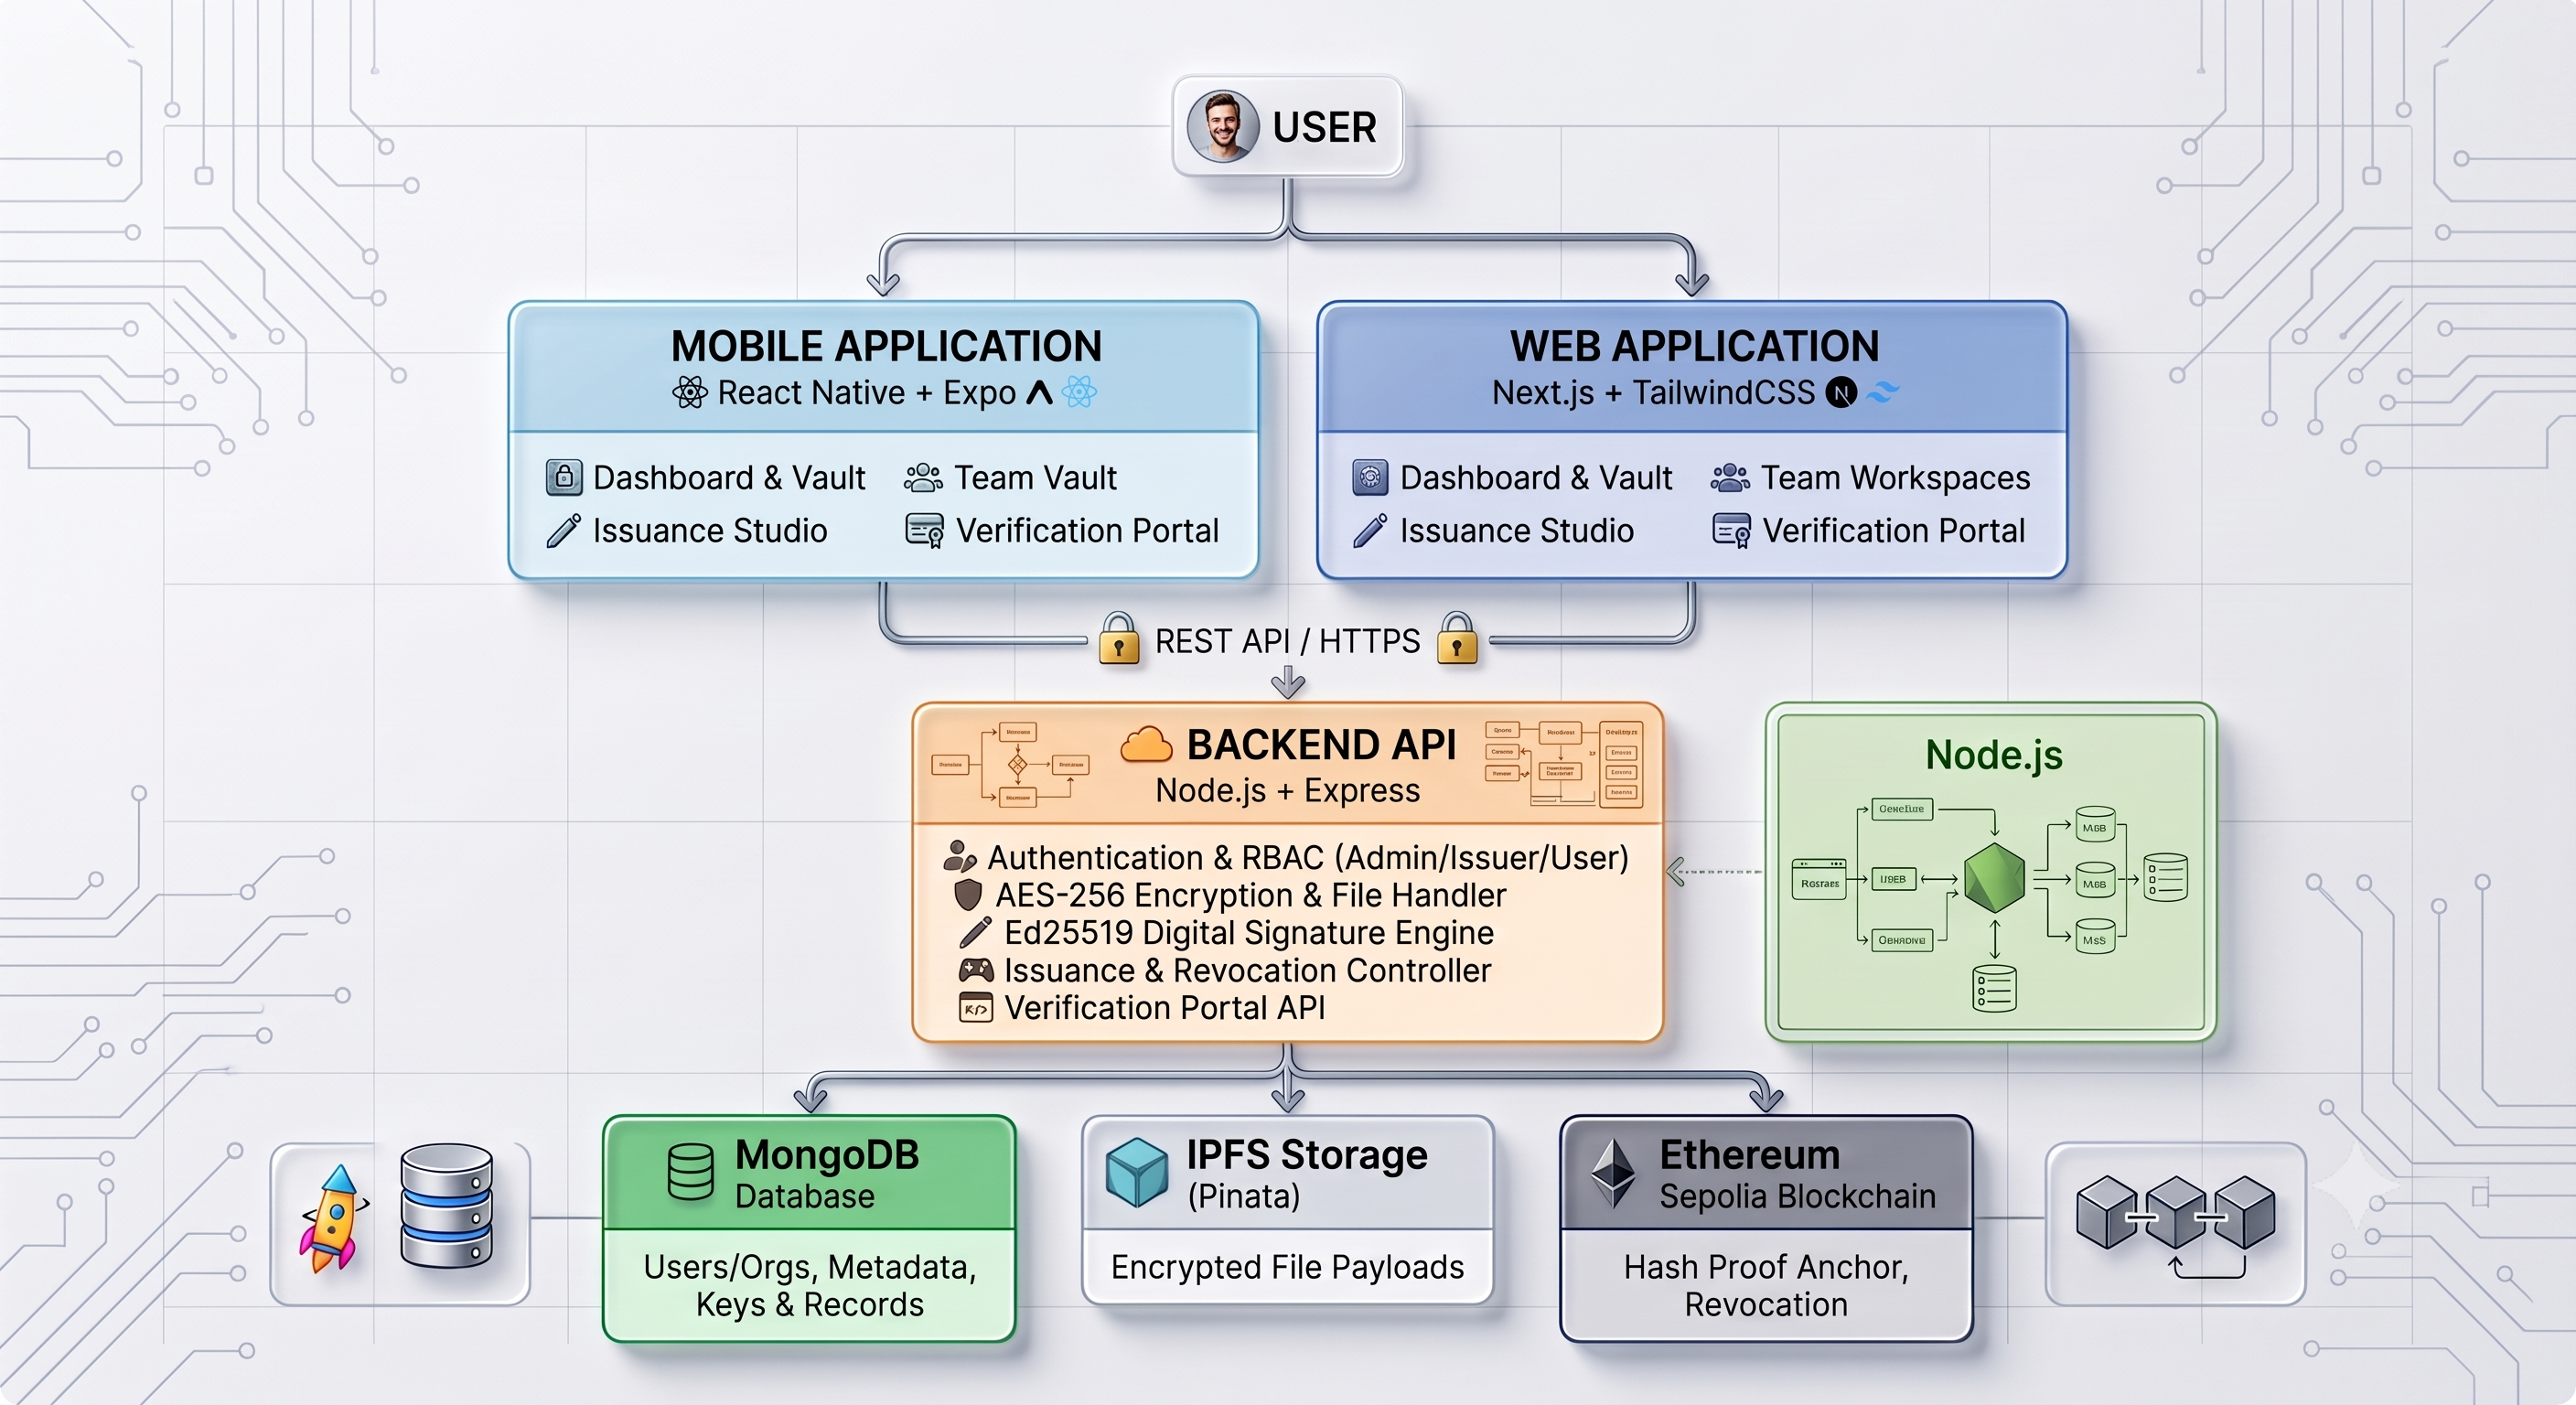
\includegraphics[width=0.95\textwidth]{Figure1.png}
    \caption{System Architecture of the Secure Document Vault}
    \label{fig:system_architecture}
\end{figure}

The system begins with the \textbf{User}, who can access the platform through either the mobile application or the web application. The mobile application is developed using \textbf{React Native with Expo}, while the web application is developed using \textbf{Next.js with TailwindCSS}. Both applications provide document-management and organizational features such as the dashboard and vault, organization directory, and verification functionality. The mobile and web applications also provide additional system-specific features such as team vaults, team workspaces, and issuance functionality.

Both applications communicate with the backend through \textbf{REST APIs over HTTPS}. The backend is implemented using \textbf{Node.js and Express} and acts as the central processing layer of the system. It manages authentication and role-based access control for \textbf{Admin, Issuer, and User} roles. It also handles file processing and \textbf{AES-256 encryption}, digital signatures using the \textbf{Ed25519} signature engine, issuance and revocation operations, and APIs required by the verification portal.

The backend communicates with three major storage and verification components. \textbf{MongoDB} is used to store users, organizations, metadata, keys, and other system records. \textbf{IPFS Storage through Pinata} is used to store encrypted file payloads. The \textbf{Ethereum Sepolia Blockchain} provides a blockchain-based integrity layer by maintaining hash proof anchors and revocation information.

This architecture separates the user interfaces from the backend processing and storage layers. It allows the mobile application developed as part of the Major Project to use the existing backend infrastructure while providing mobile users with secure document-management, access-control, search, organization, and controlled document-access functionality.


% =========================================================
\subsection{System Use Case Diagram}

The System Use Case Diagram illustrates the major interactions between different types of users and the Secure Document Vault. It identifies four primary actors: \textbf{User, Authorized Issuer, Organization Admin, and Public Verifier}. Each actor has a different set of operations based on their responsibilities and access privileges.

\begin{figure}[H]
    \centering
    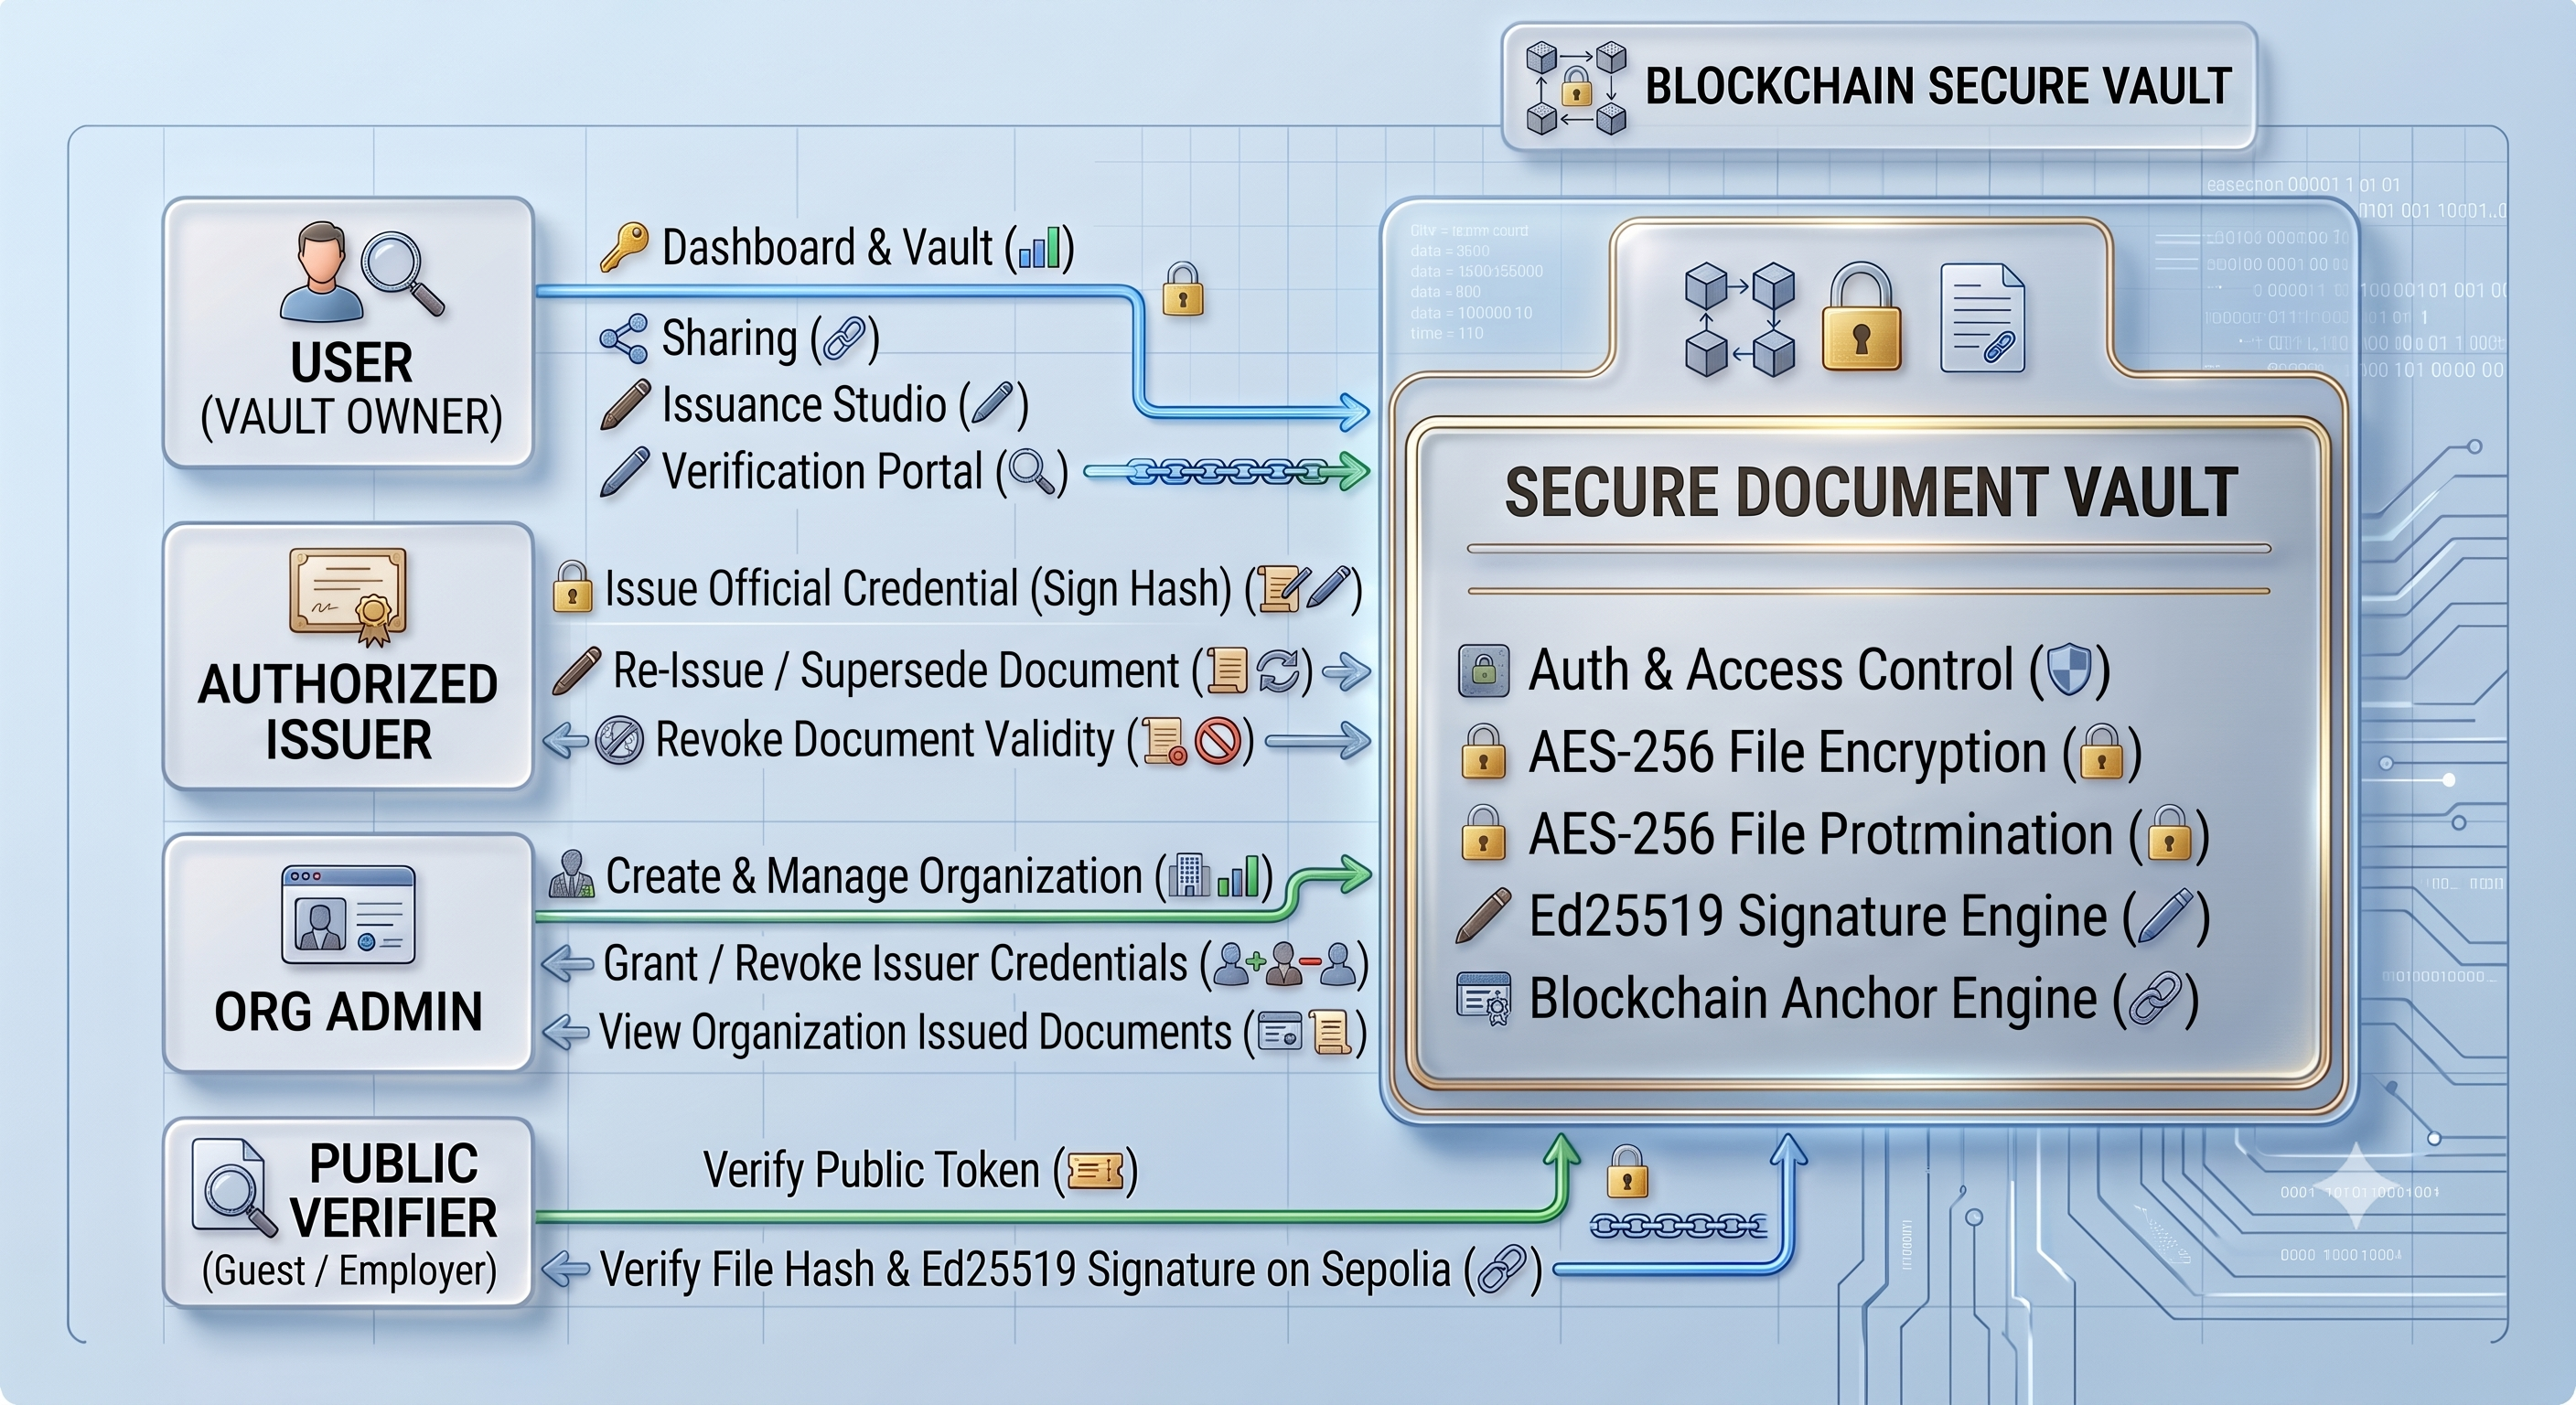
\includegraphics[width=0.95\textwidth]{Figure2.png}
    \caption{System Use Case Diagram}
    \label{fig:use_case}
\end{figure}

The \textbf{User} is the primary system user and can register and authenticate, upload and encrypt personal files, view documents stored in the personal vault, share documents, and view received credentials. These operations represent the basic document-management and credential-related functionality available to users.

The \textbf{Authorized Issuer} is responsible for issuing and managing official credentials. The issuer can issue an official credential by signing the document hash, re-issue or supersede an existing document, and revoke the validity of a document when required.

The \textbf{Organization Admin} manages organization-level operations. The administrator can create and manage an organization, grant or revoke issuer credentials, and view documents issued by the organization.

The \textbf{Public Verifier}, which may represent a guest or employer, provides an external verification role. The verifier can verify a public token and verify the file hash and \textbf{Ed25519 digital signature} against the information anchored on the \textbf{Ethereum Sepolia blockchain}.

The use case diagram therefore defines the responsibilities of each actor and shows how access to system functionality is separated according to user roles. This role separation also supports the \textbf{role-based access control} objective of the Major Project.


% =========================================================
\subsection{DFD Level 0 (Context Diagram)}

The Level 0 Data Flow Diagram (DFD), also called the Context Diagram, provides a high-level representation of the data exchanged between the \textbf{Blockchain Secure Vault System} and its external actors and storage components. The system is represented as a single central process consisting of the \textbf{Web Application, Mobile Application, and Backend}.

\begin{figure}[H]
    \centering
    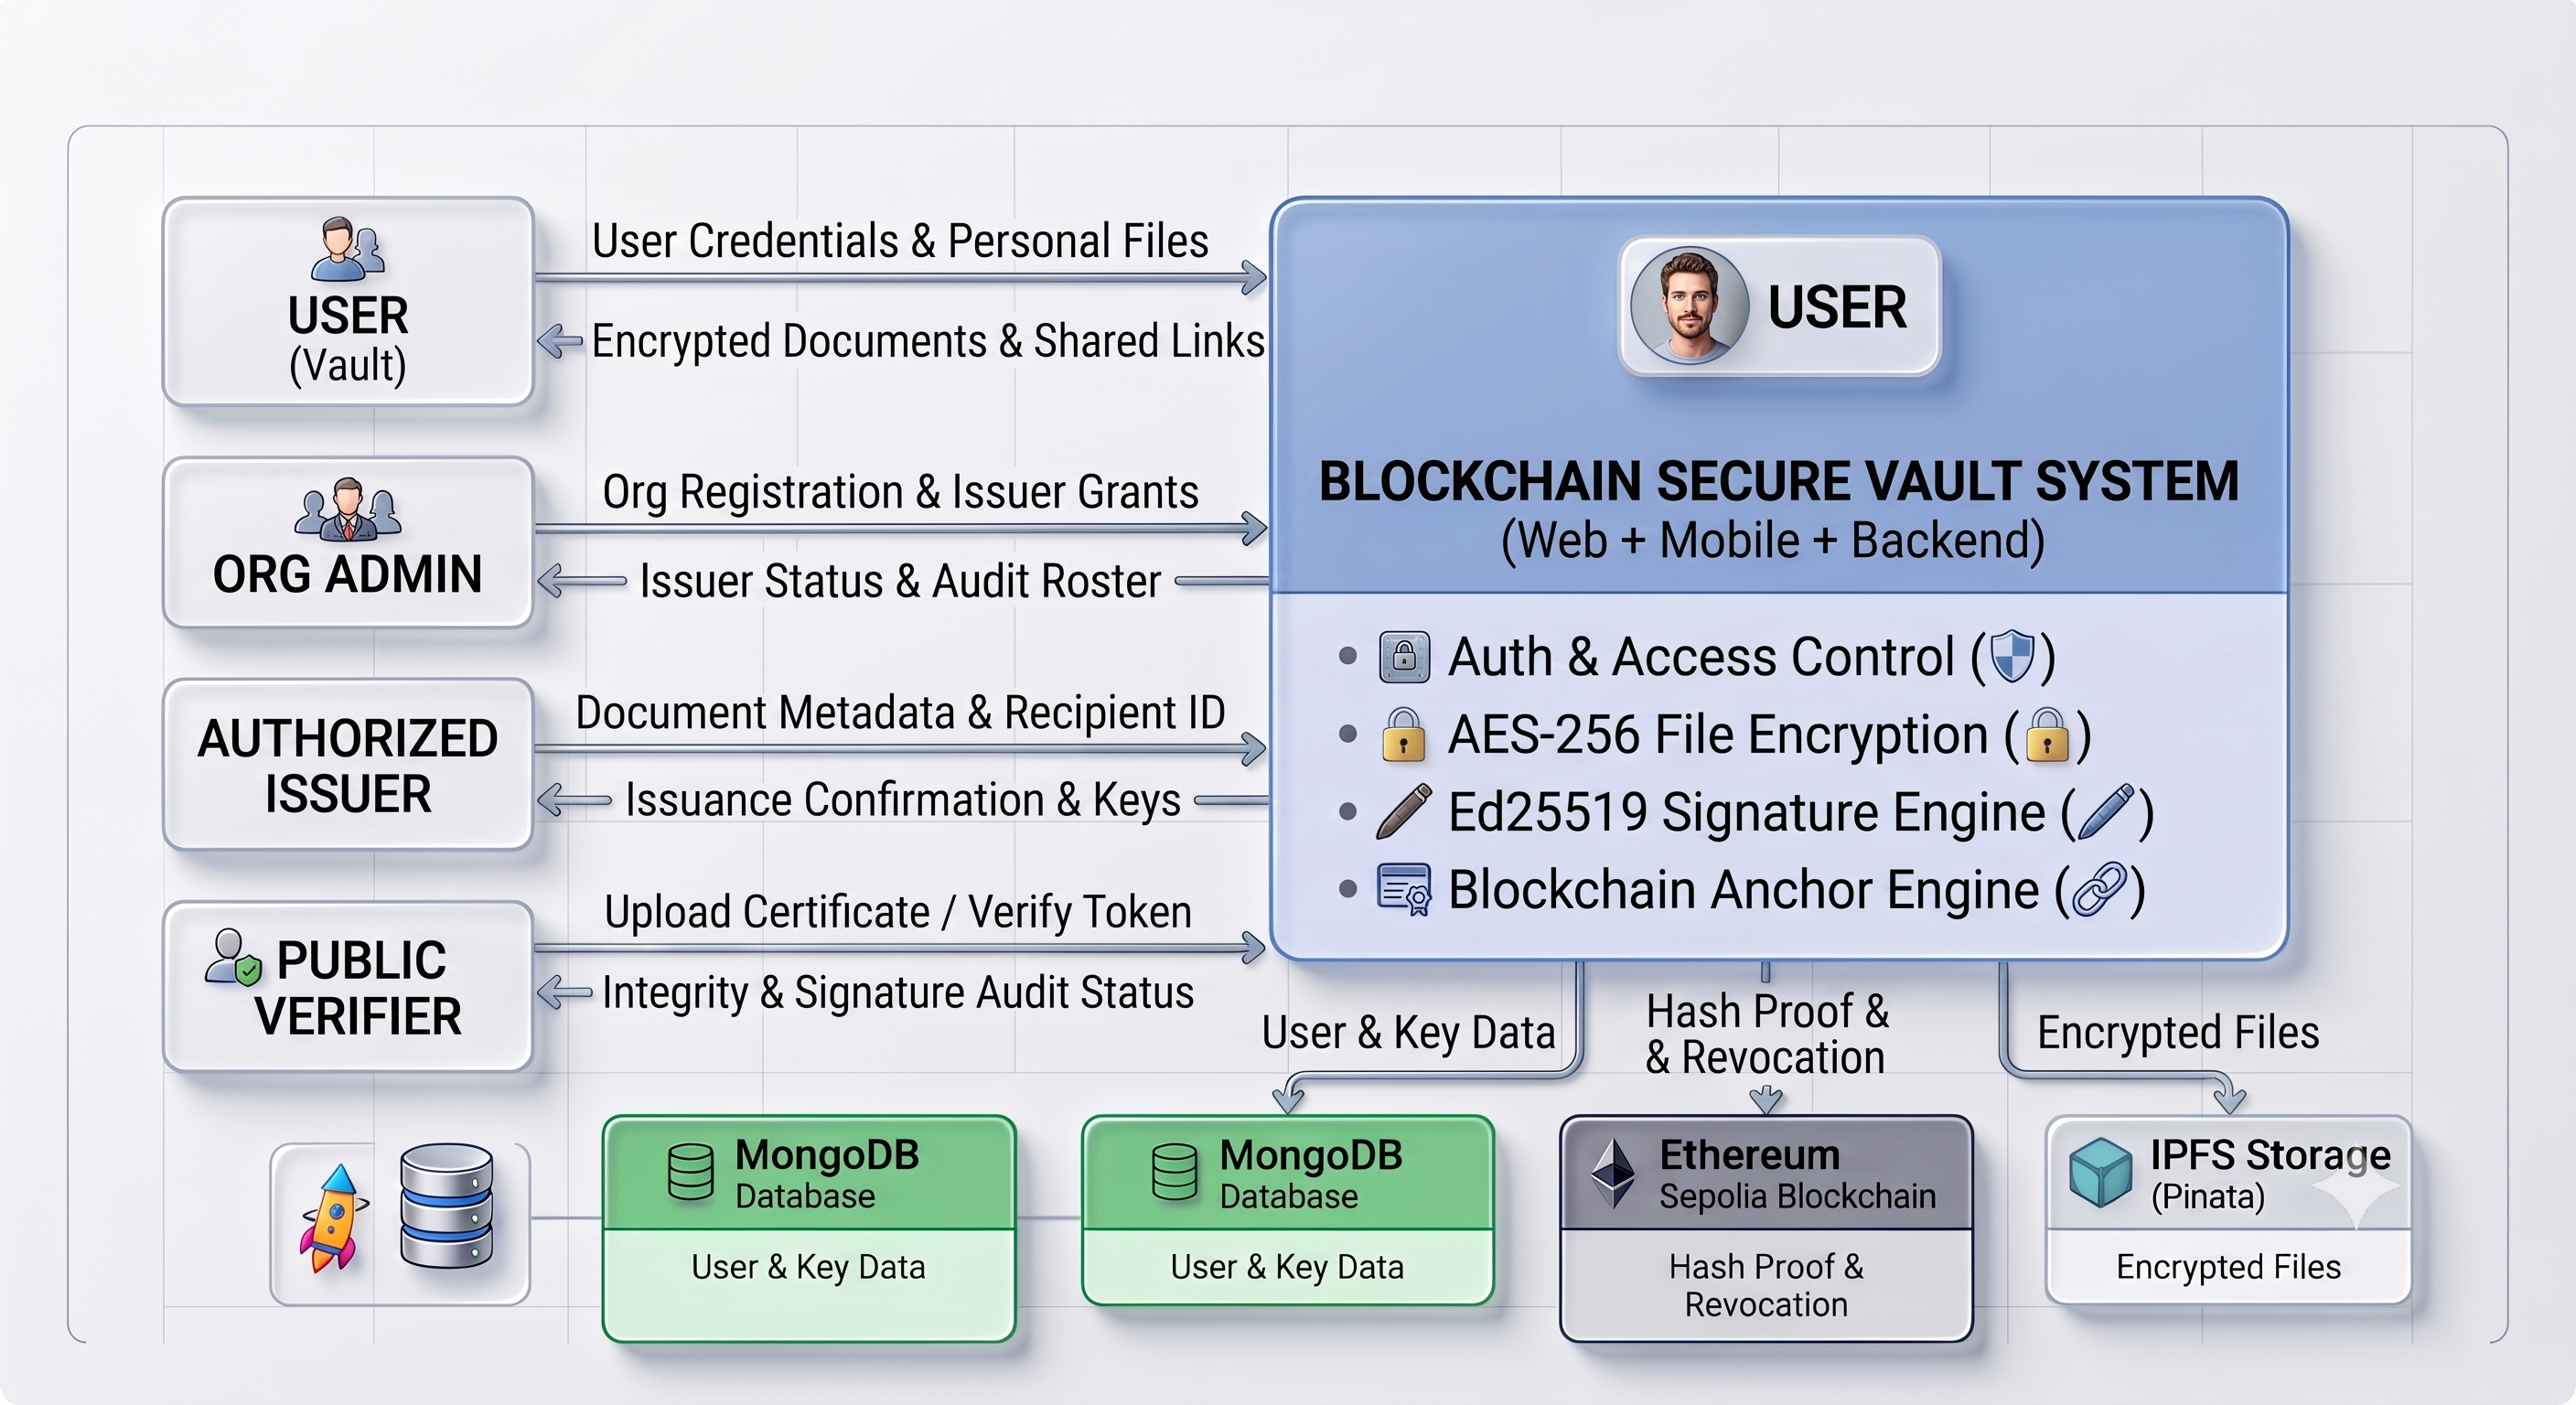
\includegraphics[width=0.95\textwidth]{Figure3.png}
    \caption{DFD Level 0 (Context Diagram)}
    \label{fig:dfd_level0}
\end{figure}

The \textbf{User (Vault)} interacts with the system by providing user credentials and personal files. In return, the system provides encrypted documents and shared links. This interaction represents the core document-management functionality of the system.

The \textbf{Organization Admin} provides organization registration information and issuer grants to the system. The system returns issuer status and the organization audit roster. This interaction represents organization-level administration and access management.

The \textbf{Authorized Issuer} provides document metadata and recipient information to the system. The system responds with issuance confirmation and relevant keys. This supports the controlled issuance and management of official documents.

The \textbf{Public Verifier} provides a certificate or verification token to the system for verification. The system returns the integrity and signature audit status, allowing the verifier to determine whether the submitted document information is valid.

The central system also communicates with three supporting storage and verification components. \textbf{MongoDB} stores user and key data, \textbf{Ethereum Sepolia Blockchain} stores hash proofs and revocation information, and \textbf{IPFS Storage through Pinata} stores encrypted files.

The DFD therefore provides a high-level view of the major data flows without describing the internal processing steps of the system. It establishes how users and external actors interact with the system and how the system exchanges information with its persistent storage and blockchain components.


% =========================================================
\subsection{DFD Level 1}

The Level 1 Data Flow Diagram provides a more detailed representation of the internal processing of the Blockchain Secure Vault System. It decomposes the system into five major processes: \textbf{Authentication and RBAC Control, Personal Vault and AES-256 Encryption, Organization and Issuer Management, Ed25519 Digital Signature and Issuance, and Dual-Check Public Verification Portal}.

\begin{figure}[H]
    \centering
    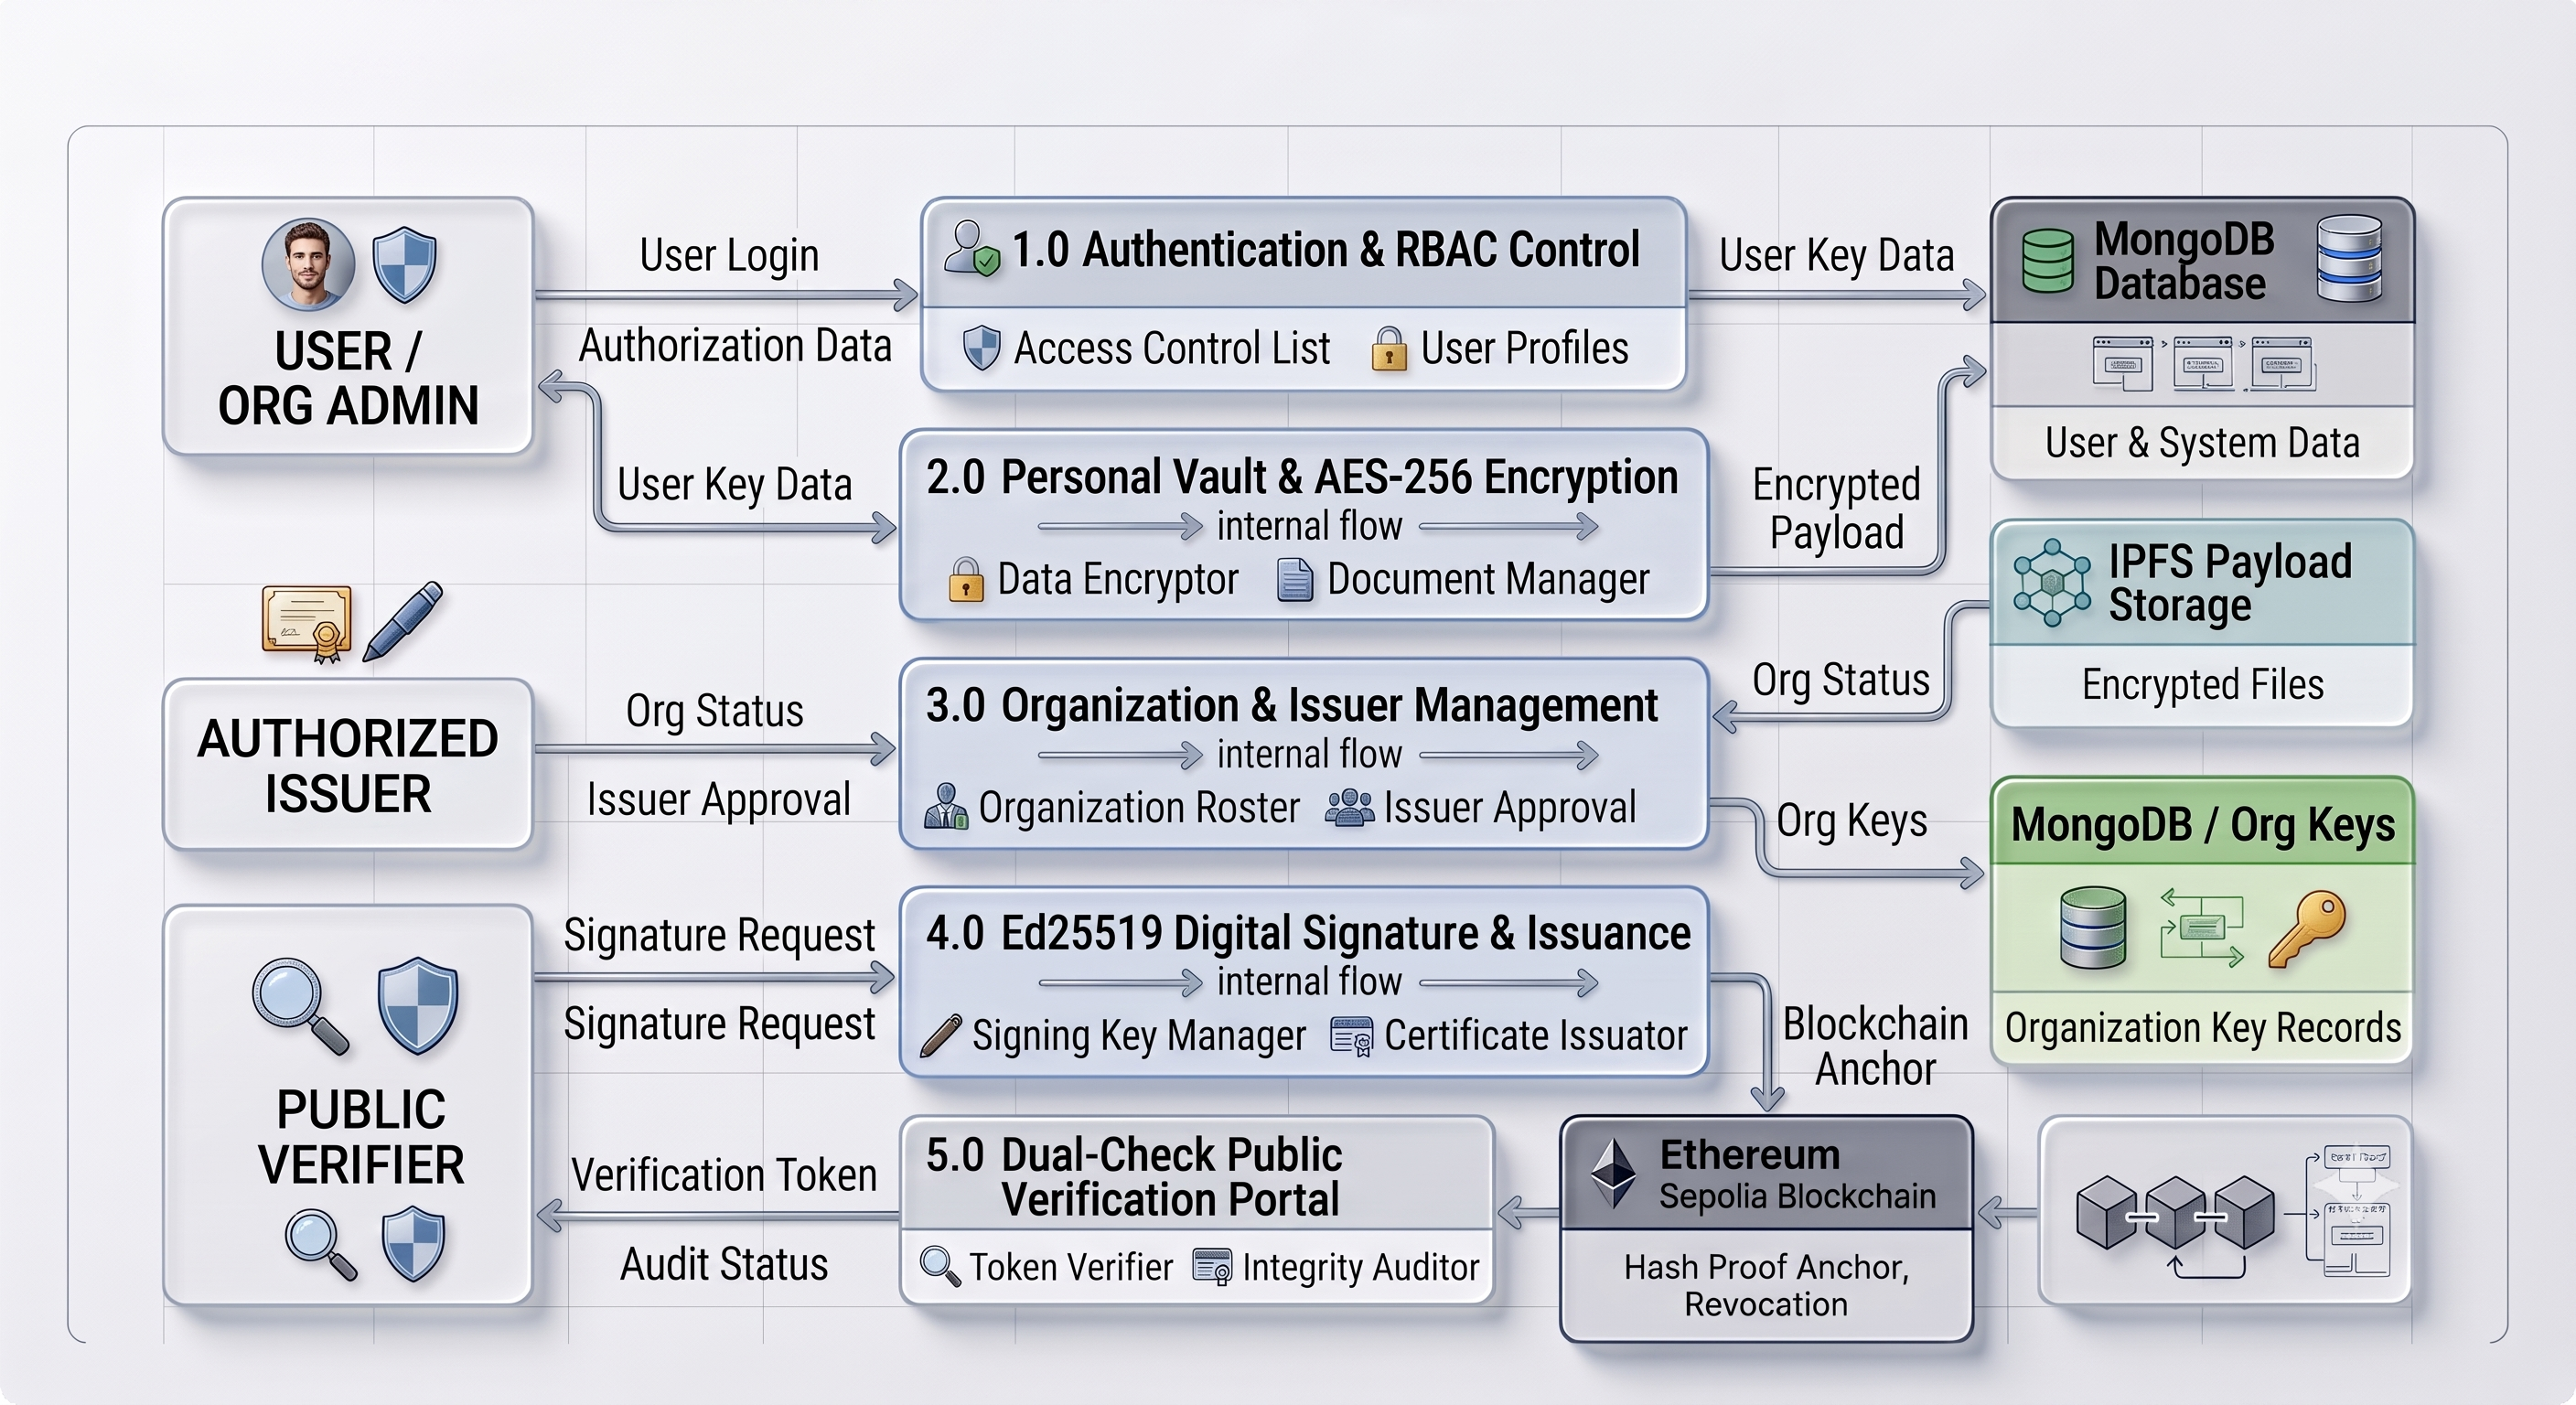
\includegraphics[width=0.95\textwidth]{Figure4.png}
    \caption{DFD Level 1 of the Blockchain Secure Vault System}
    \label{fig:dfd_level1}
\end{figure}

The first process, \textbf{1.0 Authentication \& RBAC Control}, receives authentication and access requests from the User or Organization Admin. It communicates with the \textbf{MongoDB Database} to retrieve and maintain the information required for authentication and role-based access control. This process ensures that users can access only the functions permitted by their assigned roles.

The second process, \textbf{2.0 Personal Vault \& AES-256 Encryption}, handles personal document management and file protection. After authentication and authorization, documents are processed through the personal vault and protected using \textbf{AES-256 encryption}. The encrypted payload is then stored in \textbf{IPFS Payload Storage}.

The third process, \textbf{3.0 Organization \& Issuer Management}, handles organization-level operations and issuer management. The Authorized Issuer interacts with this process, while organization-related keys and information are maintained through \textbf{MongoDB / Organization Keys}.

The fourth process, \textbf{4.0 Ed25519 Digital Signature \& Issuance}, handles digital signing and document issuance. It uses the \textbf{Ed25519 digital signature mechanism} and communicates with the \textbf{Ethereum Sepolia Blockchain} for blockchain-based anchoring and related issuance information.

The fifth process, \textbf{5.0 Dual-Check Public Verification Portal}, provides document verification functionality for the Public Verifier. The process receives verification requests and uses information from the Ethereum Sepolia Blockchain to perform the required verification checks before returning the verification result.

Overall, the Level 1 DFD shows how authentication and access control, encrypted document storage, organization management, digital signing, issuance, and public verification are connected within the system. It provides more detail than the Level 0 context diagram while still maintaining a high-level view of the major system processes.


% =========================================================
\subsection{Sequence Diagram -- Public Dual-Check Verification}

The sequence diagram illustrates the step-by-step process followed when a \textbf{Public Verifier} checks the authenticity of a document through the public verification portal. The verification process involves the \textbf{Verifier, Public Portal, Backend API, and Ethereum Sepolia Blockchain}.

\begin{figure}[H]
    \centering
    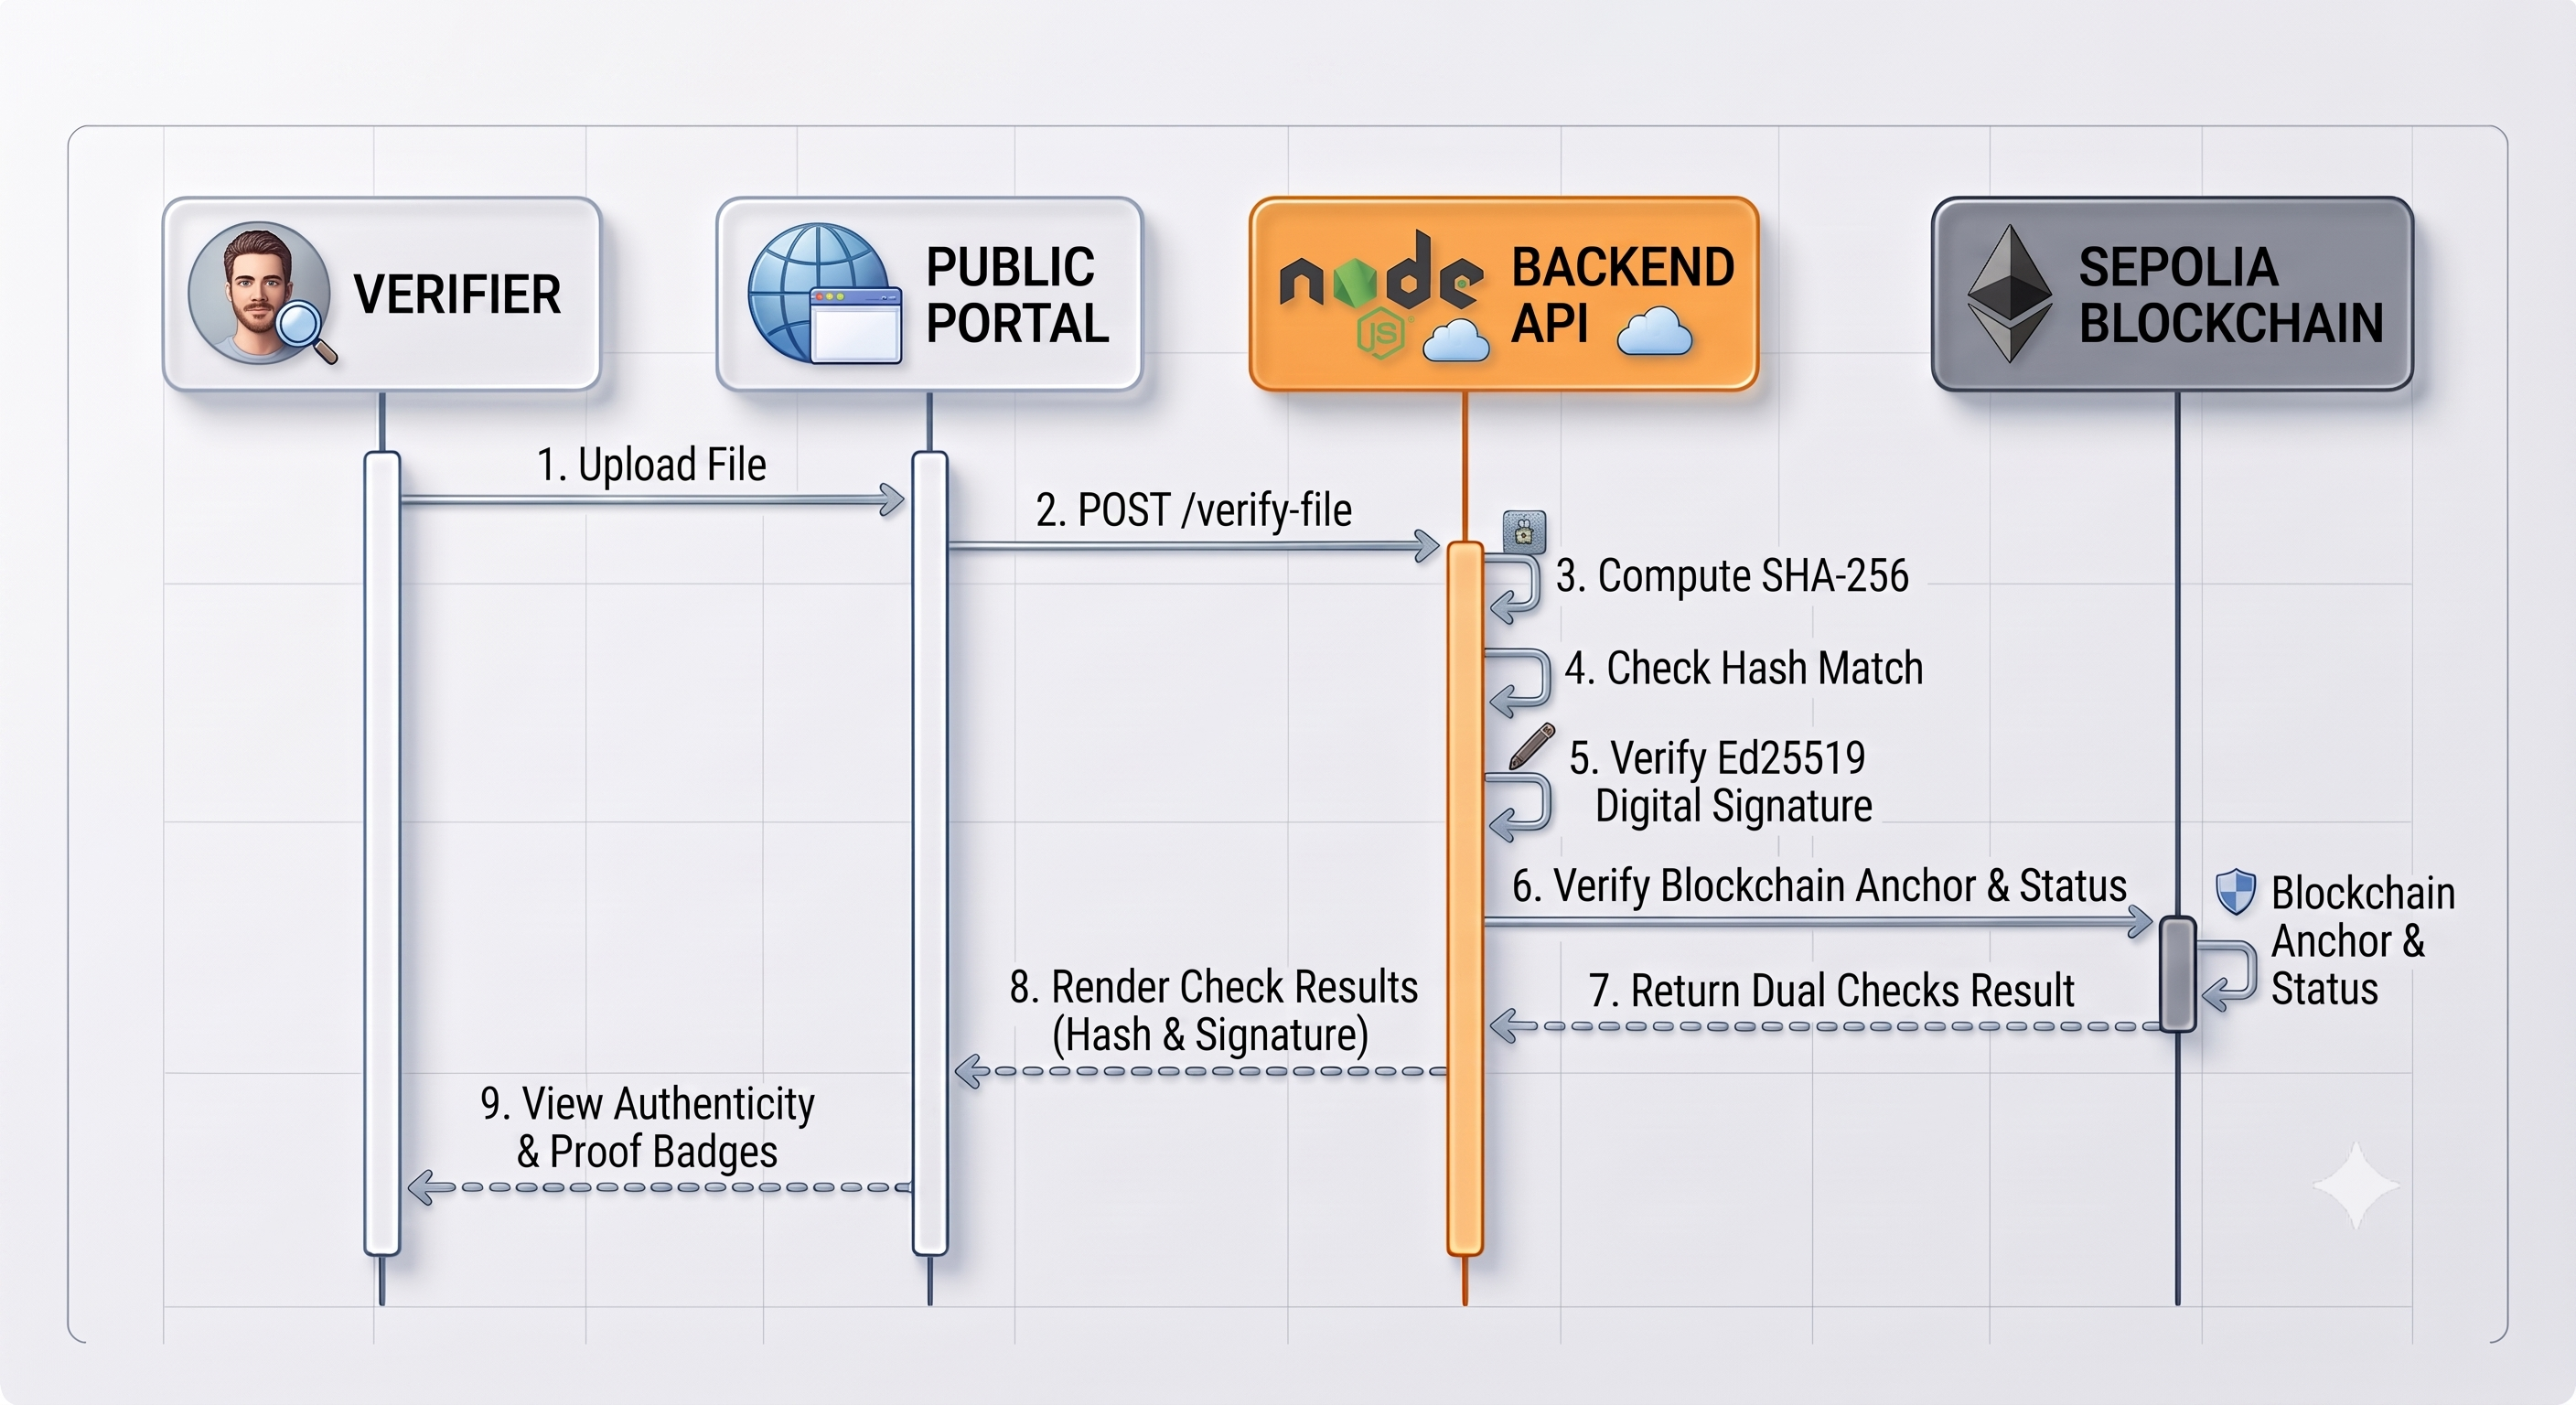
\includegraphics[width=0.95\textwidth]{Figure5.png}
    \caption{Sequence Diagram for Public Dual-Check Verification}
    \label{fig:sequence_verification}
\end{figure}

The process begins when the \textbf{Verifier uploads a file} through the Public Portal. The portal sends a \texttt{POST /verify-file} request to the Backend API to initiate the verification process.

The Backend API then computes the \textbf{SHA-256 hash} of the uploaded file and checks whether the calculated hash matches the expected document hash. It also verifies the \textbf{Ed25519 digital signature} associated with the document.

After performing the file-level checks, the Backend API communicates with the \textbf{Ethereum Sepolia Blockchain} to verify the blockchain anchor and the current status of the document. The blockchain response is returned to the backend, which combines the results of the hash, digital signature, and blockchain checks.

The Backend API then returns the \textbf{dual-check verification result} to the Public Portal. The portal renders the verification results, including the hash and signature checks, for the verifier. Finally, the verifier can view the document's \textbf{authenticity status and proof badges}.

This sequence demonstrates how the verification process combines file-level integrity checking with digital-signature and blockchain verification to provide an authenticity result to an external verifier.


% =========================================================
\subsection{Activity Diagram -- Controlled Document Access \& Decryption}

The activity diagram represents the workflow followed when an authenticated user attempts to access a document from the personal vault. It focuses on the authorization check performed before the encrypted document is retrieved and decrypted.

\begin{figure}[H]
    \centering
    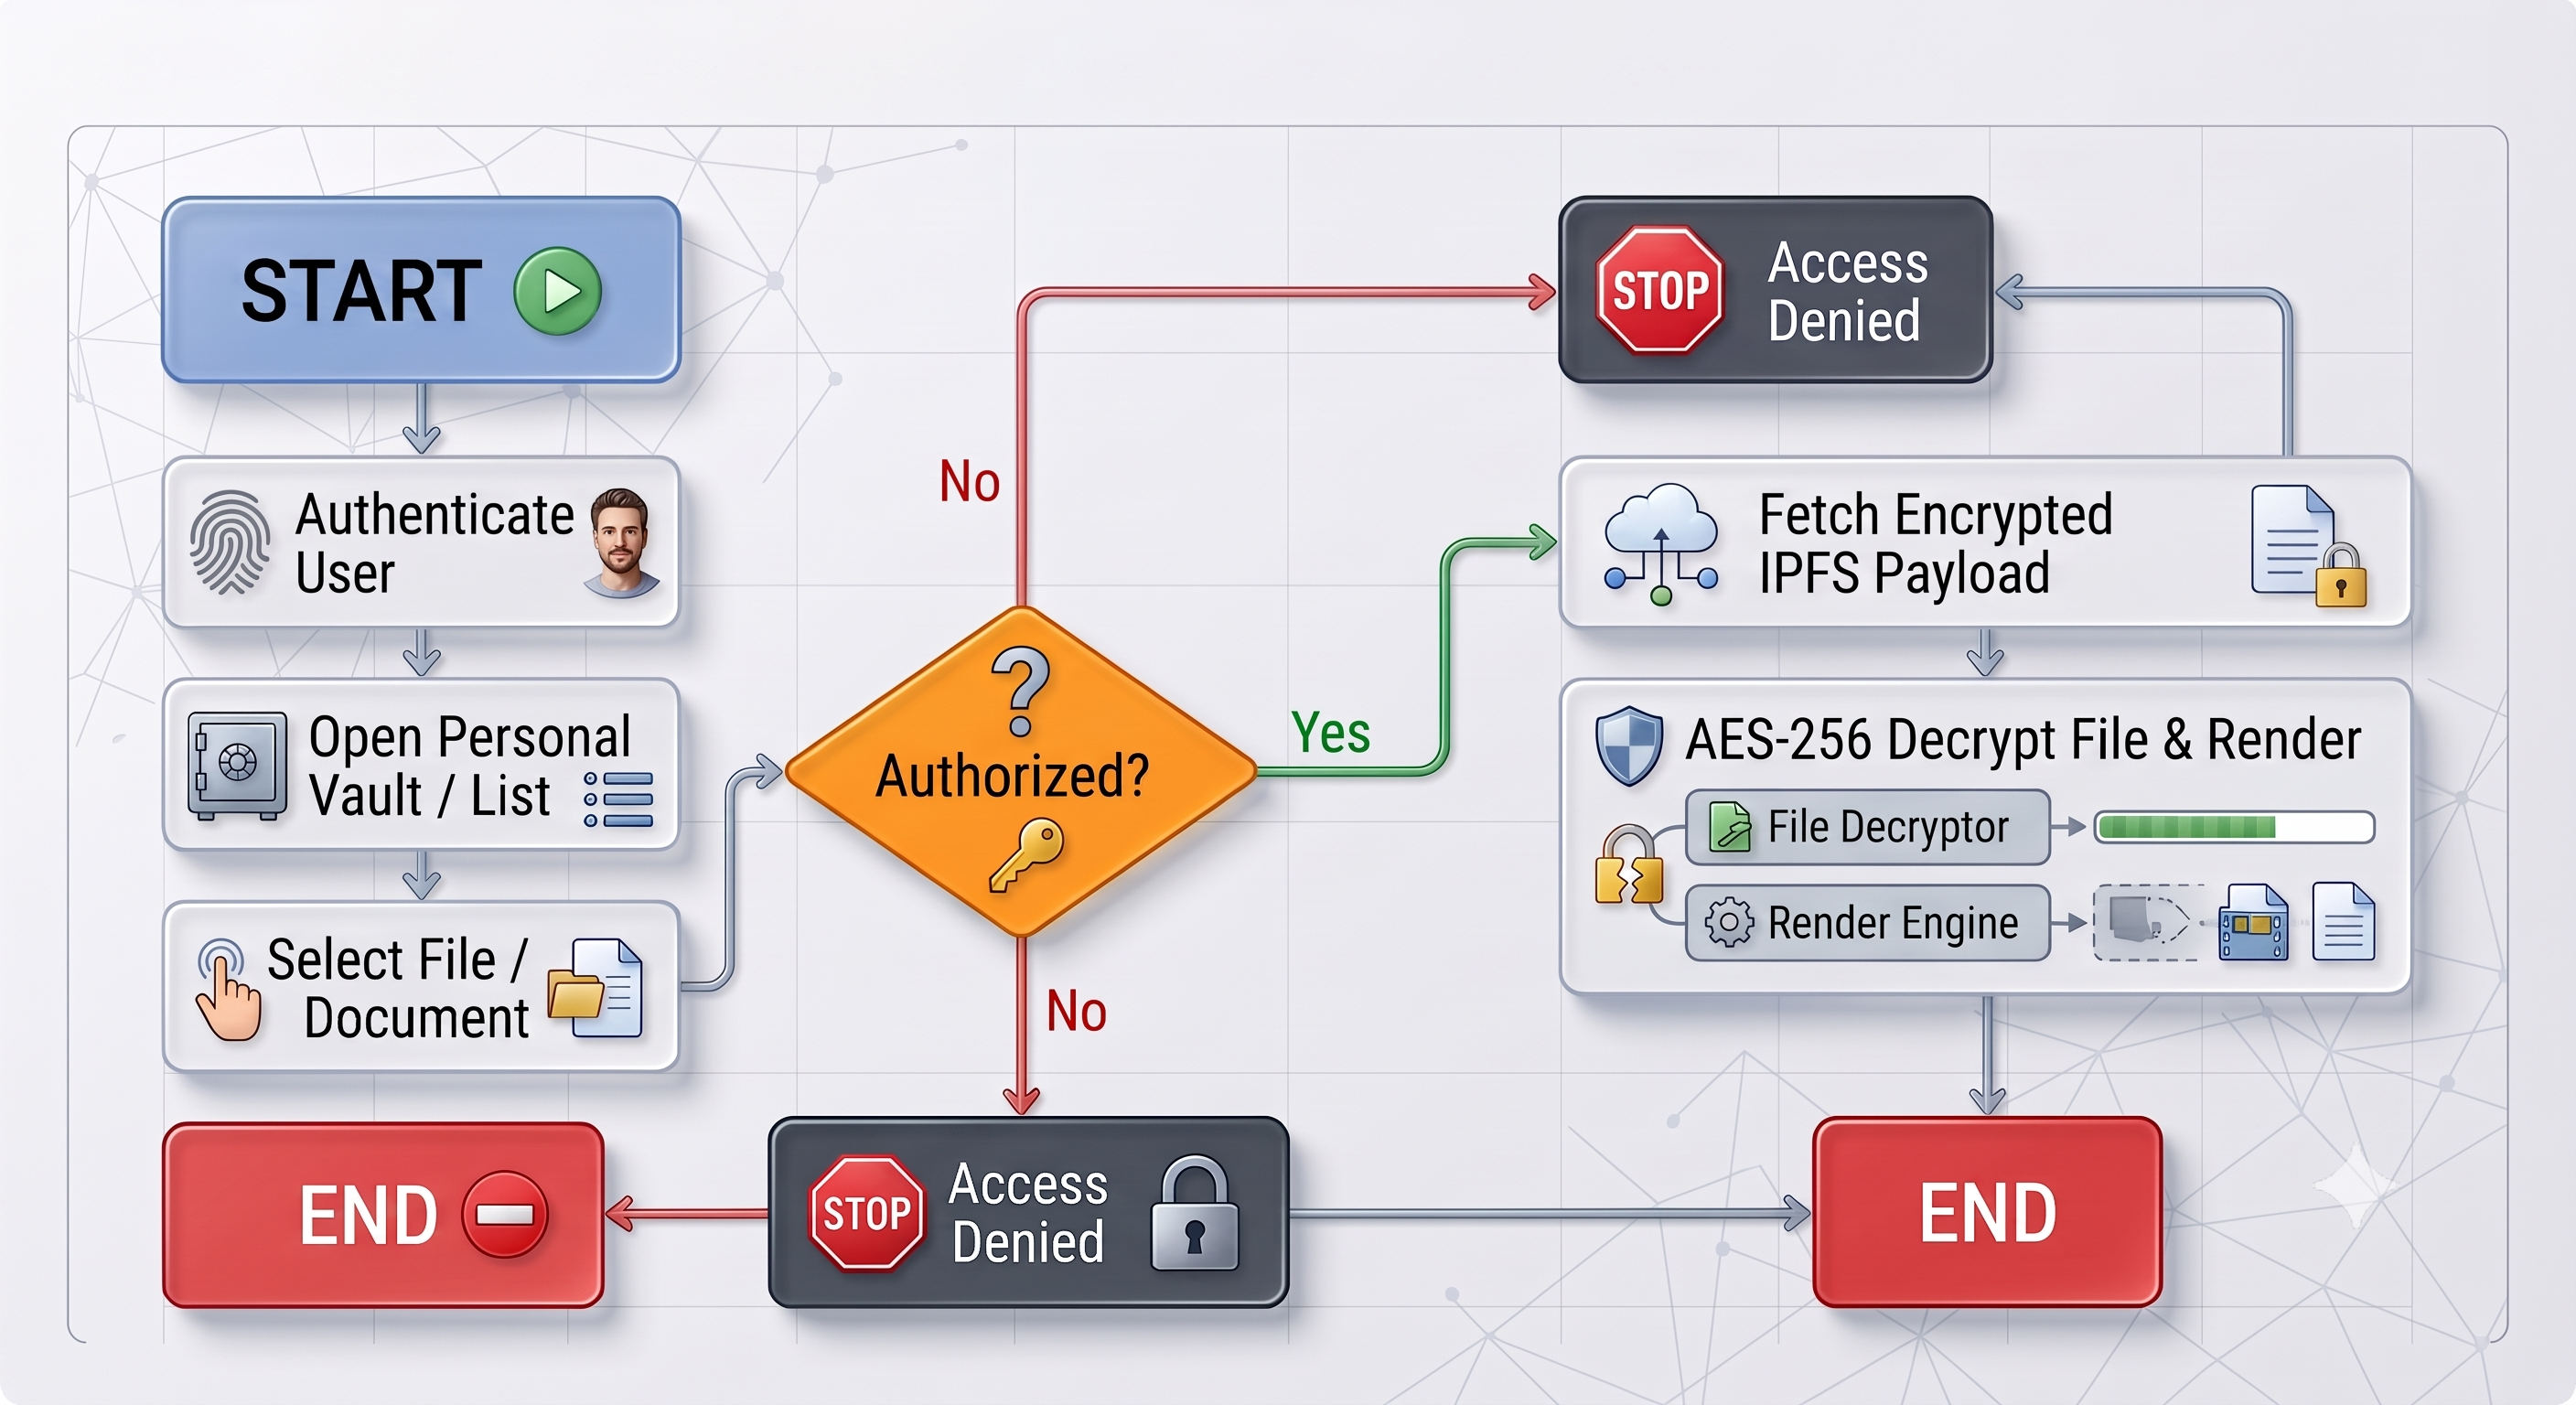
\includegraphics[width=0.95\textwidth]{Figure6.png}
    \caption{Activity Diagram for Controlled Document Access and Decryption}
    \label{fig:activity_document_access}
\end{figure}

The process begins when the user \textbf{authenticates} with the system. After successful authentication, the user opens the \textbf{Personal Vault} and views the available documents. The user then selects a file or document for access.

The system performs an \textbf{authorization check} to determine whether the user is permitted to access the selected document. If the user is not authorized, the system generates an \textbf{Access Denied} response and terminates the access workflow.

If the user is authorized, the system retrieves the \textbf{encrypted IPFS payload} associated with the selected document. The encrypted file is then processed using \textbf{AES-256 decryption}, after which the decrypted file is rendered for the authorized user.

The workflow ensures that document access is controlled before the encrypted file is retrieved and displayed. This supports secure document access by combining authorization checks with encrypted document storage and controlled decryption.


% =========================================================
\subsection{Class / Entity Diagram}

The Class / Entity Diagram represents the major data entities involved in the Secure Document Vault and the relationships between them. The diagram focuses on users, organizations, issuer authorization, documents, issuance records, and document-sharing links.

\begin{figure}[H]
    \centering
    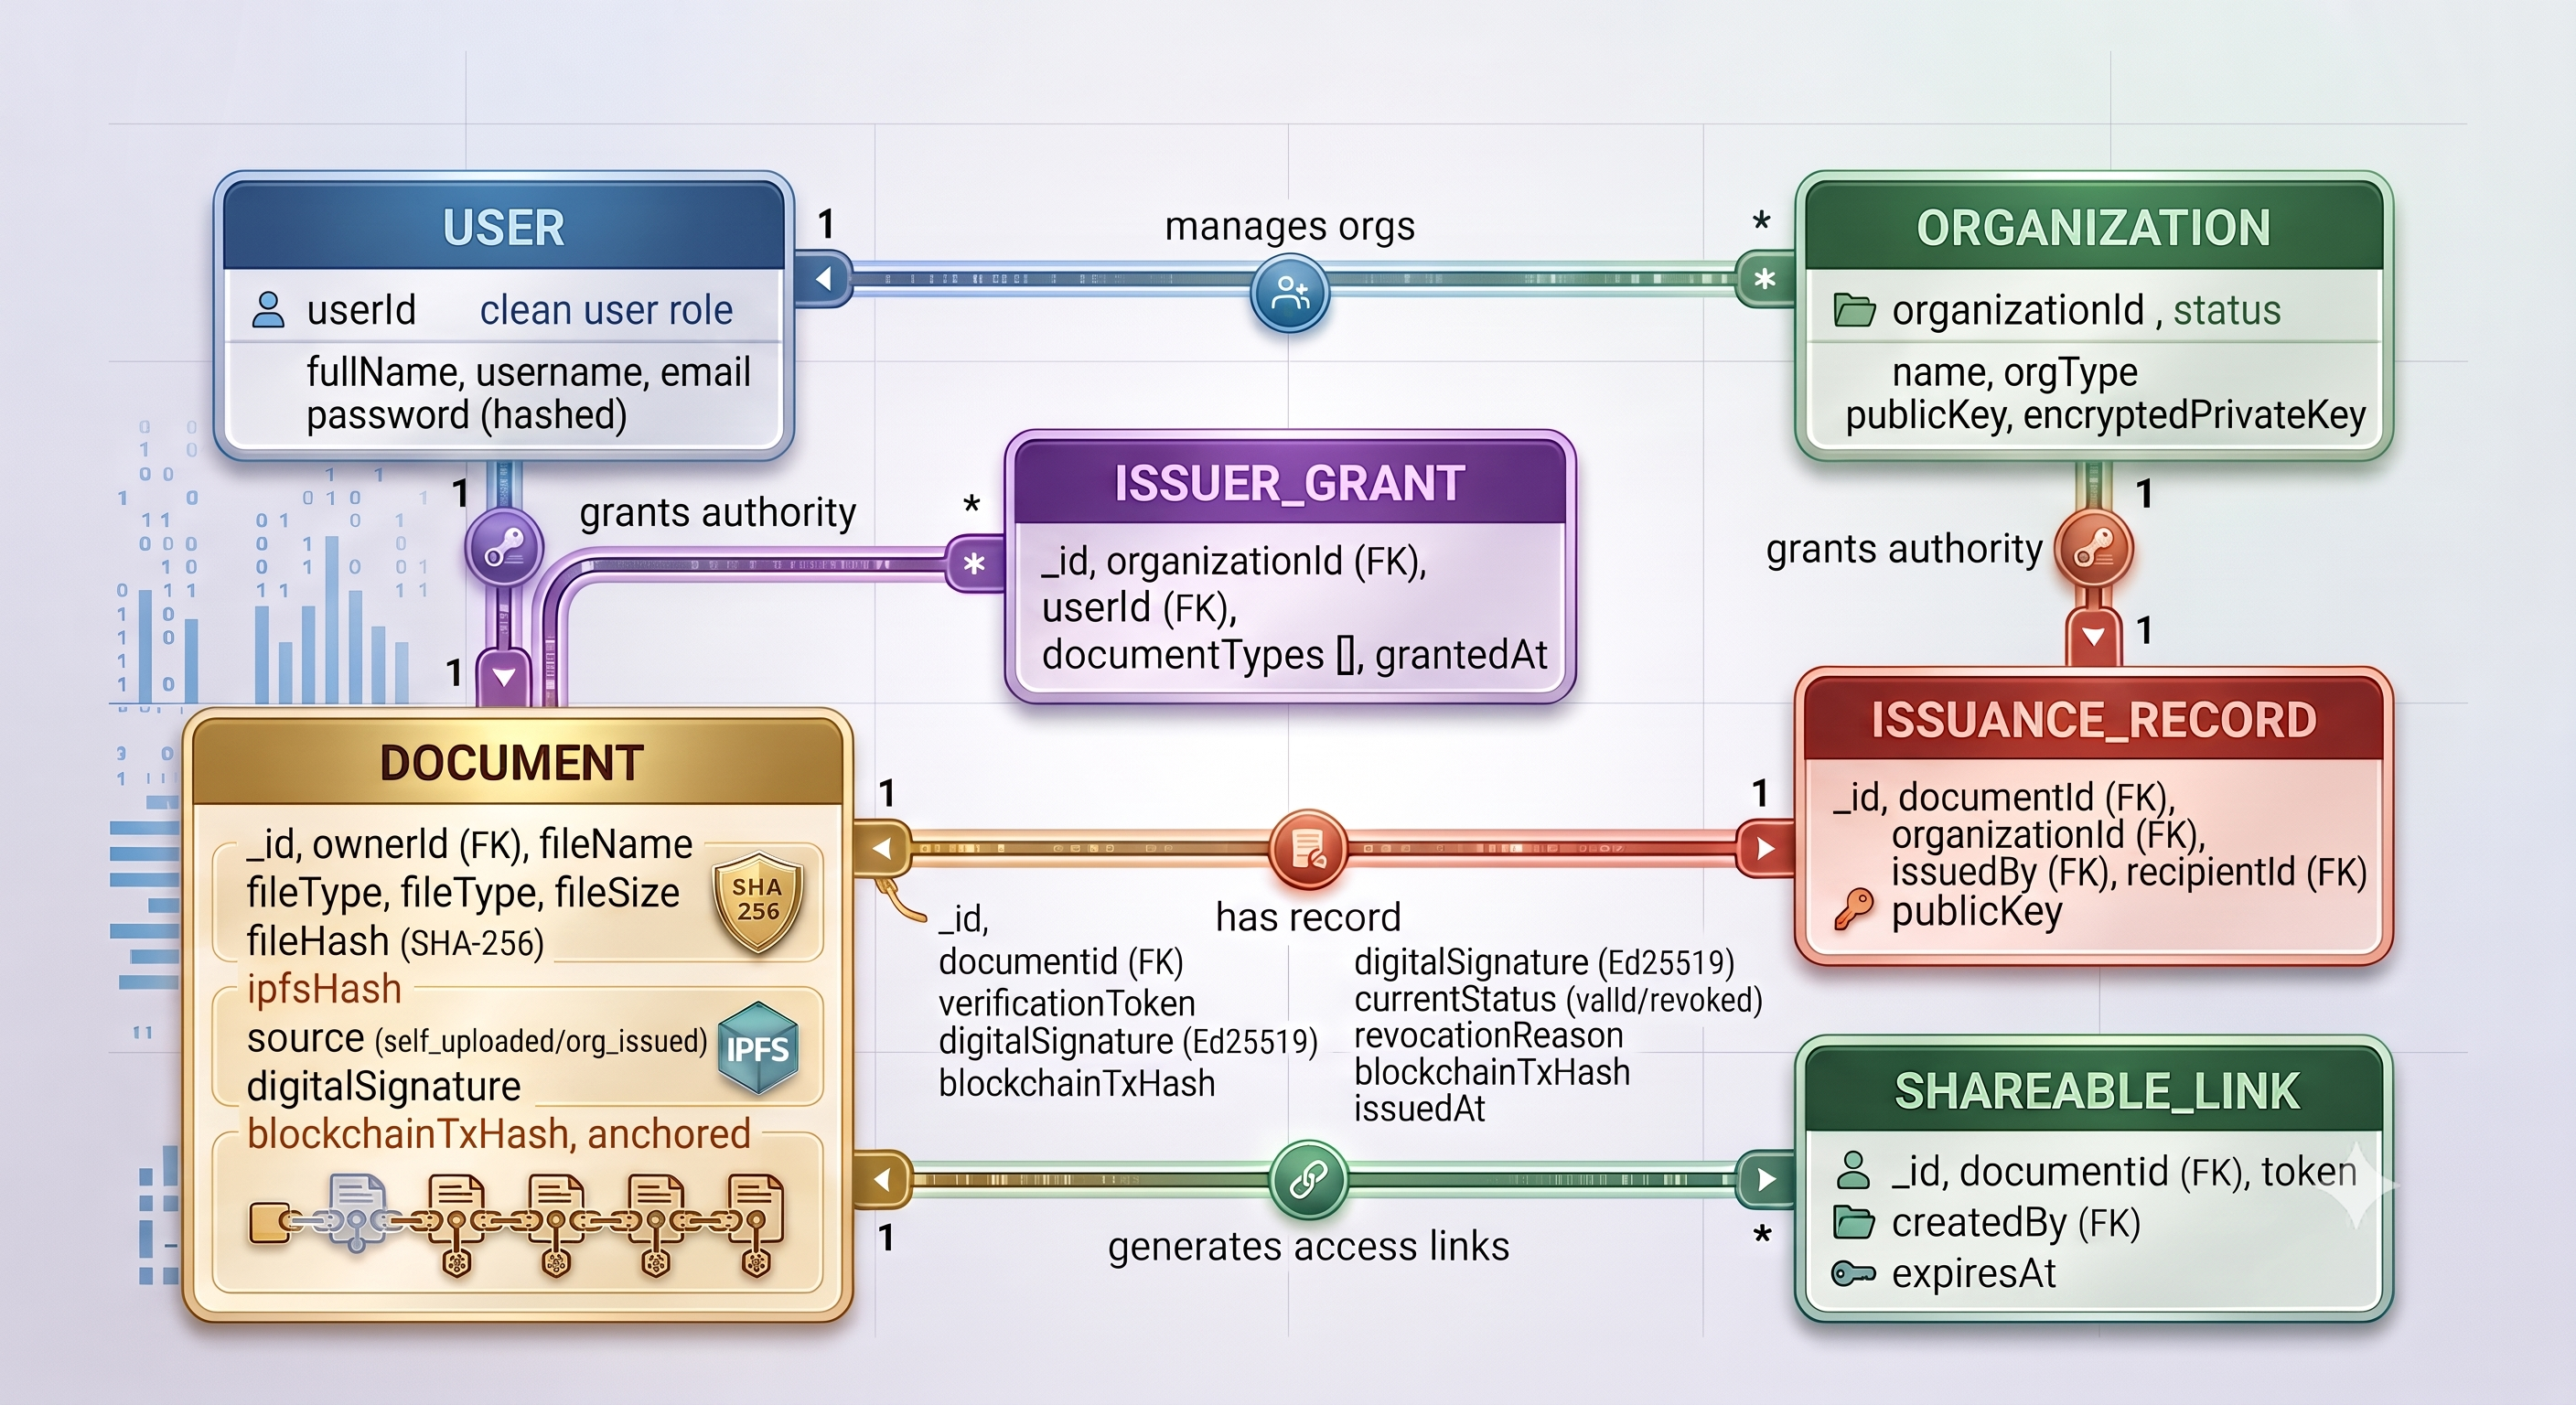
\includegraphics[width=0.95\textwidth]{Figure7.png}
    \caption{Class / Entity Diagram of the Secure Document Vault}
    \label{fig:class_entity}
\end{figure}

The \textbf{User} entity stores information related to system users, including their identity details, hashed password, and assigned role. A user can manage organizations and can be associated with organization-level authority.

The \textbf{Organization} entity represents an organization registered within the system. It contains organization information, status, and cryptographic key information. Organizations are connected with users through organizational management and issuer authority.

The \textbf{Issuer Grant} entity represents the authority granted to a user to perform issuer-related operations within an organization. It records the organization, user, permitted document types, and the time at which the authority was granted.

The \textbf{Document} entity represents files managed by the system. It stores information such as the owner, file name, file type, file size, \textbf{SHA-256 file hash}, IPFS hash, document source, digital signature, and blockchain transaction information. These attributes support document identification, integrity verification, and secure storage.

The \textbf{Issuance Record} entity maintains information about documents issued by an organization. It contains the document and organization references, issuer and recipient information, verification token, \textbf{Ed25519 digital signature}, current document status, revocation information, blockchain transaction hash, and issuance timestamp.

The \textbf{Shareable Link} entity represents an access link generated for sharing a document. It maintains the associated document, access token, creator information, and expiration time. This allows document access to be shared through controlled and potentially time-limited links.

The relationships shown in the diagram establish how users, organizations, documents, issuer permissions, issuance records, and shareable links are connected. These relationships provide the underlying data structure required for document ownership, organizational issuance, authorization, and controlled document sharing.


% =========================================================
\subsection{Deployment Diagram}

The Deployment Diagram represents the physical and runtime arrangement of the major components of the Secure Document Vault. It shows how the \textbf{mobile client, web client, backend server, database, decentralized storage, and blockchain network} are connected during system operation.

\begin{figure}[H]
    \centering
    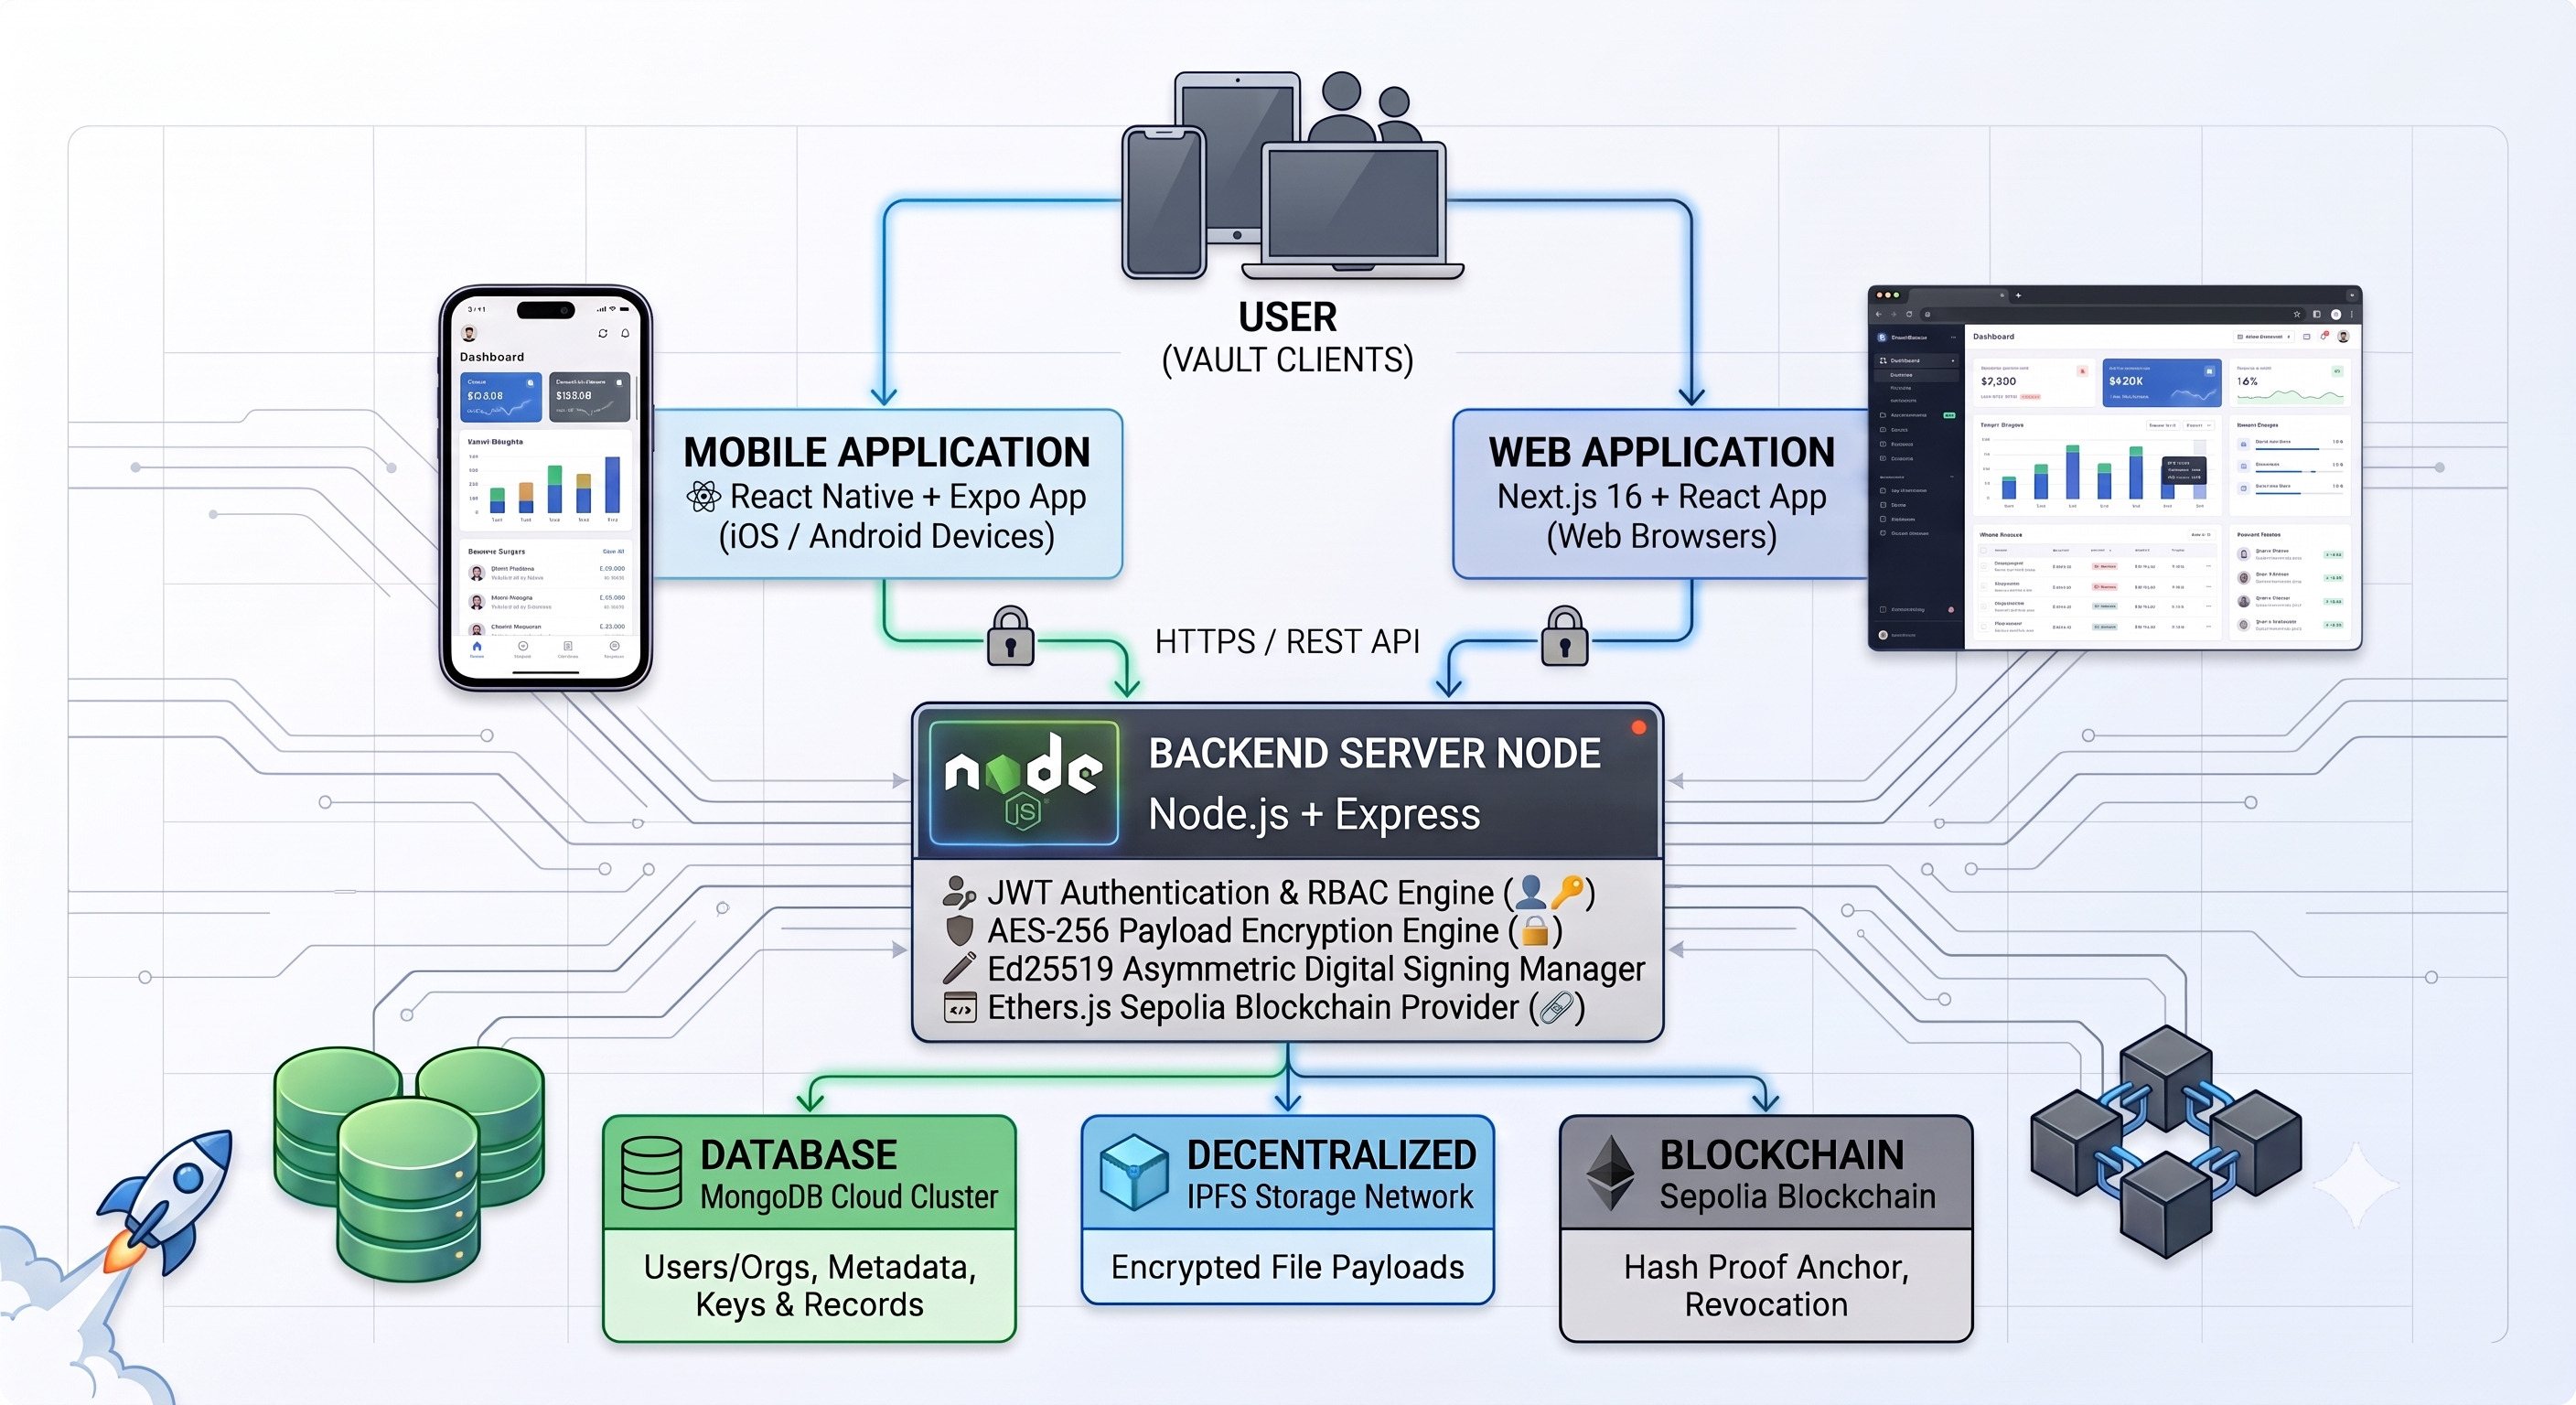
\includegraphics[width=0.95\textwidth]{Figure8.png}
    \caption{Deployment Diagram of the Secure Document Vault}
    \label{fig:deployment}
\end{figure}

The \textbf{Mobile Client Node} represents mobile devices running the application developed using \textbf{React Native and Expo}. The application can operate on iOS and Android devices and provides mobile access to the document vault and other system functionality.

The \textbf{Web Client Node} represents web browsers running the \textbf{Next.js and React} application. Both the mobile and web clients communicate with the backend server through \textbf{HTTPS using REST APIs}.

The \textbf{Backend Server Node} hosts the Node.js and Express runtime and contains the main server-side processing components. These include the \textbf{JWT Authentication and RBAC Engine}, \textbf{AES-256 Payload Encryption Engine}, \textbf{Ed25519 Asymmetric Digital Signing Manager}, and the \textbf{Ethers.js Sepolia Blockchain Provider}.

The backend server communicates with three external infrastructure nodes. The \textbf{Database Node} contains the MongoDB Cloud Cluster for persistent application data. The \textbf{Decentralized Node} represents the IPFS storage network used for decentralized file storage. The \textbf{Blockchain Node} represents the Ethereum Sepolia network used for blockchain-based document verification and related blockchain operations.

The deployment structure separates client applications, backend processing, persistent database storage, decentralized file storage, and blockchain services. This separation allows the mobile and web applications to access the same backend services while maintaining dedicated infrastructure for data storage, encrypted file storage, and blockchain-based verification.


% =========================================================
\subsection{Design Summary}

The software design provides a structured representation of the Secure Document Vault from multiple perspectives. The \textbf{System Architecture} describes the major application, backend, storage, and blockchain components and their communication. The \textbf{Use Case Diagram} defines the responsibilities and interactions of the User, Authorized Issuer, Organization Admin, and Public Verifier.

The \textbf{DFD Level 0} provides a high-level representation of the data exchanged between the system and its external actors, while the \textbf{DFD Level 1} further decomposes the system into authentication, document encryption, organization management, digital signing and issuance, and public verification processes.

The \textbf{Sequence Diagram} demonstrates the public document verification workflow, including SHA-256 hash calculation, Ed25519 signature verification, and blockchain-anchor verification. The \textbf{Activity Diagram} demonstrates controlled document access, where authorization is checked before encrypted content is retrieved and decrypted.

The \textbf{Class / Entity Diagram} represents the main data entities and their relationships, including users, organizations, issuer grants, documents, issuance records, and shareable links. Finally, the \textbf{Deployment Diagram} shows how the mobile and web clients communicate with the backend server and how the backend interacts with MongoDB, IPFS, and Ethereum Sepolia.

Together, these diagrams provide a comprehensive design view of the system while supporting the Major Project objectives related to \textbf{secure mobile document management, role-based access control, document organization and sharing, and controlled document access and verification}.


\newpage

\section{Testing Module}

Testing is an important part of the Major Project because the mobile application handles document management and controlled access to potentially sensitive information. The testing process is used to verify that the implemented functionality works according to the specified requirements and that unauthorized users cannot access protected operations.



% ---------------------------------------------------------
\subsection{Testing Objectives}

The main objectives of testing are:

\begin{itemize}
    \item To verify that the mobile application functions correctly.
    \item To verify communication between the mobile application and backend APIs.
    \item To verify that authenticated users can access authorized functionality.
    \item To verify role-based access restrictions.
    \item To verify document retrieval and search functionality.
    \item To verify document viewing and sharing operations.
    \item To identify errors in the application and correct them during development.
    \item To ensure that partially developed functionality is clearly identified rather than treated as complete.
\end{itemize}


% ---------------------------------------------------------
\subsection{Testing Techniques}

The following testing techniques are applicable to the Major Project.


% ---------------------------------------------------------
\subsubsection{Functional Testing}

Functional testing verifies whether individual features perform their intended operations.

The major functionality tested includes:

\begin{itemize}
    \item User authentication
    \item Mobile navigation
    \item Document retrieval
    \item Document search
    \item Document viewing
    \item Document sharing
    \item Role-based access
    \item API communication
    \item Access-denied scenarios
\end{itemize}


% ---------------------------------------------------------
\subsubsection{Integration Testing}

Integration testing verifies the interaction between different components of the system.

For the Major Project, the primary integration points are:

\begin{itemize}
    \item \textbf{Mobile Application $\rightarrow$ Backend API}
    \item \textbf{Backend API $\rightarrow$ Database}
    \item \textbf{Backend API $\rightarrow$ Existing Document Services}
\end{itemize}

The purpose is to ensure that requests generated by the mobile application are correctly processed by the backend and that appropriate responses are returned.


% ---------------------------------------------------------
\subsubsection{Access-Control Testing}

Access-control testing is particularly important because one of the Major Project objectives is Role-Based Access Control.

The testing verifies that:

\begin{itemize}
    \item An authenticated user can access permitted operations.
    \item A user without the required permission cannot perform restricted operations.
    \item Organization or role-based restrictions are correctly applied.
    \item Document sharing is limited according to authorization rules.
    \item Protected API requests are rejected when authentication or authorization requirements are not satisfied.
\end{itemize}

The existing project contains JWT validation and organization/membership-based authorization mechanisms.


% ---------------------------------------------------------
\subsubsection{User Interface Testing}

The mobile interface is tested to verify:

\begin{itemize}
    \item Correct navigation between screens.
    \item Correct display of document information.
    \item Proper response to user actions.
    \item Correct handling of loading states.
    \item Appropriate display of errors and access-denied messages.
    \item Usability of document-management operations.
\end{itemize}


% ---------------------------------------------------------
\subsection{Test Cases}

The following test cases represent the main functionality relevant to the Major Project.
\begin{table}[H]
\centering
\caption{Test Cases for the Major Project}
\label{tab:test_cases}
\renewcommand{\arraystretch}{1.35}
\begin{tabular}{|c|p{3.0cm}|p{4.0cm}|p{5.3cm}|}
\hline
\textbf{Test Case ID} &
\textbf{Test Scenario} &
\textbf{Input / Action} &
\textbf{Expected Result} \\ \hline

TC-01 &
User Login &
Enter valid login credentials &
User is authenticated and allowed to access the application \\ \hline

TC-02 &
Invalid Login &
Enter invalid credentials &
Login request is rejected and an error is displayed \\ \hline

TC-03 &
Document Retrieval &
Open document section as an authorized user &
Authorized documents are displayed \\ \hline

TC-04 &
Document Search &
Search using a document-related query &
Relevant documents are retrieved \\ \hline

TC-05 &
Unauthorized Document Access &
Attempt to access a restricted document &
Access is denied \\ \hline

TC-06 &
Role-Based Access &
Perform an operation with an unauthorized role &
Operation is rejected \\ \hline

TC-07 &
Document Sharing &
Share a document with an authorized user &
Sharing request is processed according to permissions \\ \hline

TC-08 &
Document Viewing &
Open an accessible document &
Document is displayed through the permitted viewing mechanism \\ \hline

TC-09 &
API Communication &
Perform a document operation from mobile app &
Request reaches backend and appropriate response is returned \\ \hline

TC-10 &
Invalid API Request &
Send an invalid or unauthorized request &
Backend rejects the request appropriately \\ \hline

TC-11 &
Navigation &
Move between relevant mobile screens &
Correct destination screen is displayed \\ \hline

TC-12 &
Folder/File Organization &
Create or use available organization functionality &
Documents are organized according to the implemented functionality \\ \hline

\end{tabular}
\end{table}


% ---------------------------------------------------------
\subsection{Security Testing}

Security testing focuses on preventing unauthorized access to documents and protected application functionality.

The following scenarios are considered:

\begin{enumerate}

    \item \textbf{Authentication Validation}

    Requests to protected resources should require valid authentication.

    \item \textbf{Authorization Validation}

    Authentication alone should not provide access to operations that require additional permissions.

    \item \textbf{Role Validation}

    User roles and organizational membership should be considered when processing restricted operations.

    \item \textbf{Unauthorized Access}

    Attempts to access documents without the required permissions should be rejected.

    \item \textbf{Session Security}

    Authentication information used by the mobile application should be handled using appropriate secure storage mechanisms.

\end{enumerate}

The existing system includes JWT authentication, authorization middleware, token validation, and access-control checks.





% ---------------------------------------------------------
\subsection{Expected Testing Outcome}

Successful testing should demonstrate that:

\begin{itemize}
    \item The mobile application communicates correctly with the backend.
    \item Authorized users can access their permitted documents.
    \item Unauthorized users cannot perform restricted document operations.
    \item Role-based permissions are enforced.
    \item Documents can be searched and retrieved according to the implemented functionality.
    \item Documents can be viewed through the permitted application workflow.
    \item The application handles invalid requests and errors appropriately.
    \item The remaining folder-based organization functionality can be verified after its implementation is completed.
\end{itemize}

Thus, the testing process provides a systematic method for validating the Major Project objectives while identifying functionality that still requires development before the final project evaluation.

\newpage


\section{Performance of Project Developed So Far}

The performance evaluation of the Major Project focuses on the functionality developed up to the mid-term stage. Since the project is an extension of the existing Secure Document Vault, the evaluation primarily considers the performance of the newly developed mobile application, its communication with the backend, document-management operations, and access-control mechanisms.

At the current stage, the project provides an Expo/React Native mobile application that communicates with the existing backend through REST APIs. The repository analysis confirms that the mobile application and core document-management and access-control functionality are implemented, while file/folder management remains partially implemented.


% ---------------------------------------------------------
\subsection{Mobile Application Performance}

The mobile application provides a mobile interface for accessing the Secure Document Vault. The application communicates with the backend instead of directly accessing the database or storage services.

The separation between the mobile application and backend provides the following advantages:

\begin{itemize}
    \item The mobile application remains focused on user interaction and presentation.
    \item Existing backend business logic can be reused.
    \item Database operations remain isolated from the mobile client.
    \item Authentication and authorization can be handled centrally.
    \item Changes to the backend can be utilized by both web and mobile clients.
\end{itemize}

The project architecture confirms that the web and mobile applications communicate with the same backend API.


% ---------------------------------------------------------
\subsection{Document Management Performance}

The implemented document-management functionality allows users to retrieve and interact with documents through the application.

The existing system supports document listing, sharing, downloading, viewing, and verification operations. Document search/retrieval according to user or organization context is also identified as implemented.

The performance of these operations depends on factors such as:

\begin{itemize}
    \item Network connectivity.
    \item Backend response time.
    \item Database query processing.
    \item Document size.
    \item Storage retrieval time.
    \item Mobile device resources.
\end{itemize}

No formal benchmark data for response time or throughput is currently available in the repository. Therefore, numerical performance claims are not included in this mid-term evaluation.


% ---------------------------------------------------------
\subsection{Role-Based Access Control Performance}

Role-Based Access Control provides an additional authorization layer for protected document operations.

When a user requests a protected operation, the request is processed through the authentication and authorization mechanisms before the operation is performed. This prevents unauthorized users from directly accessing restricted resources.

The project contains JWT validation, organization-level checks, and membership-based authorization. Role-based access control is identified as an implemented requirement.

This architecture allows access decisions to be handled by the backend rather than relying only on restrictions implemented in the mobile interface.





\newpage


\section{Output Screens}
% Home Page - View 1
% Home Page - View 1
\begin{figure}[H]
    \centering
    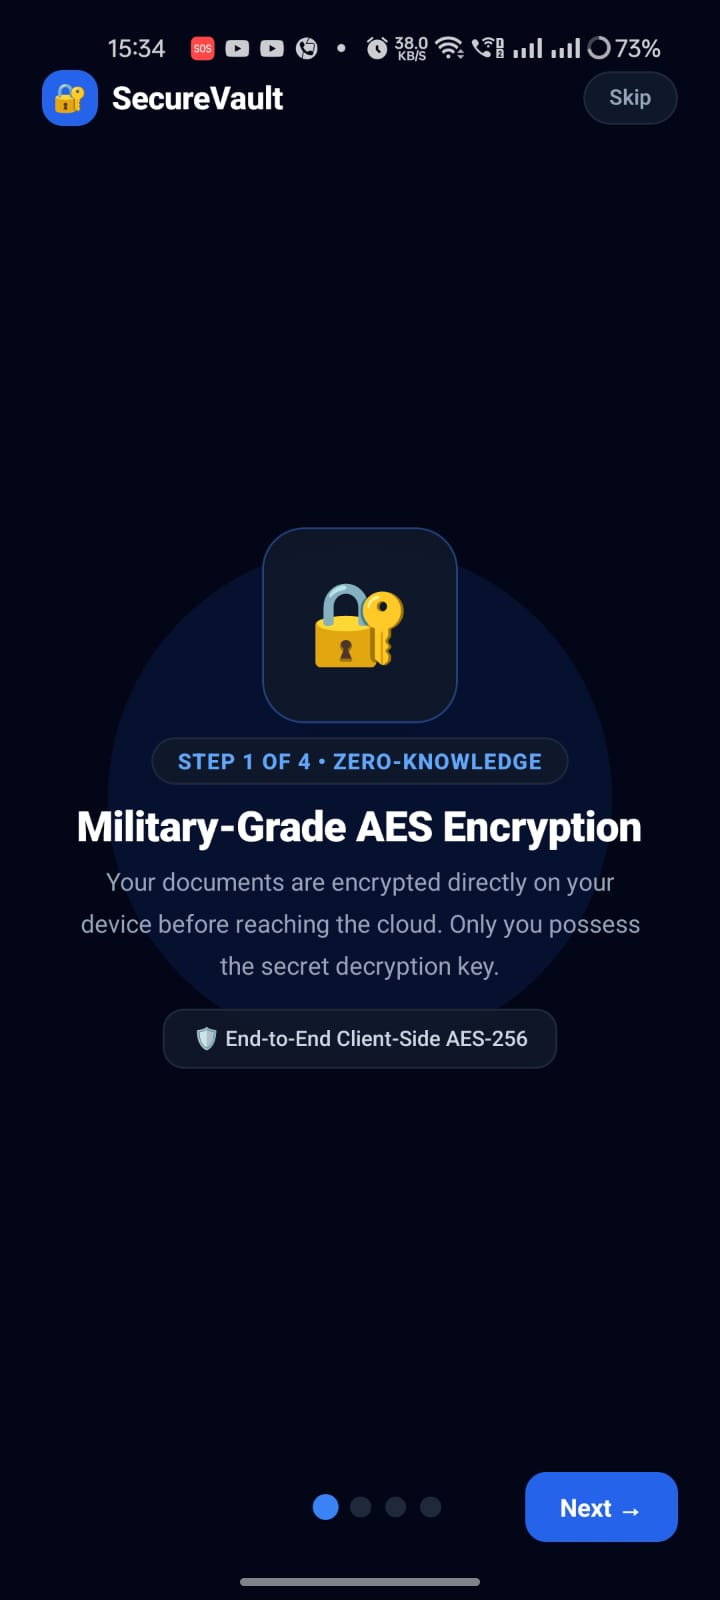
\includegraphics[width=6.5cm,height=9cm,keepaspectratio]{home1.jpeg}
    \caption{Secure Document Vault Home Page -- View 1}
    \label{fig:home-1}
\end{figure}

% Home Page - View 2
\begin{figure}[H]
    \centering
    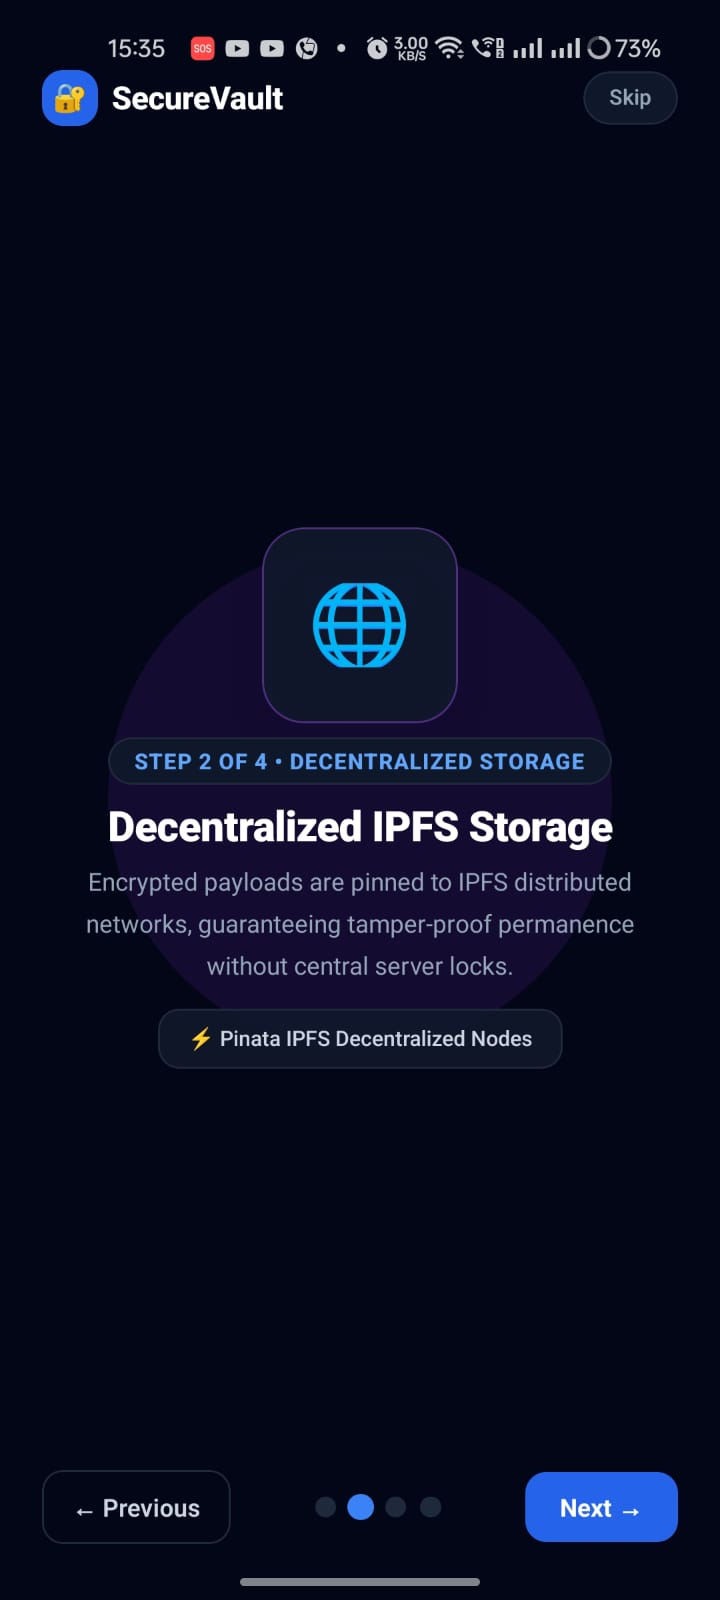
\includegraphics[width=6.5cm,height=9cm,keepaspectratio]{home2.jpeg}
    \caption{Secure Document Vault Home Page -- View 2}
    \label{fig:home-2}
\end{figure}

% Home Page - View 3
\begin{figure}[H]
    \centering
    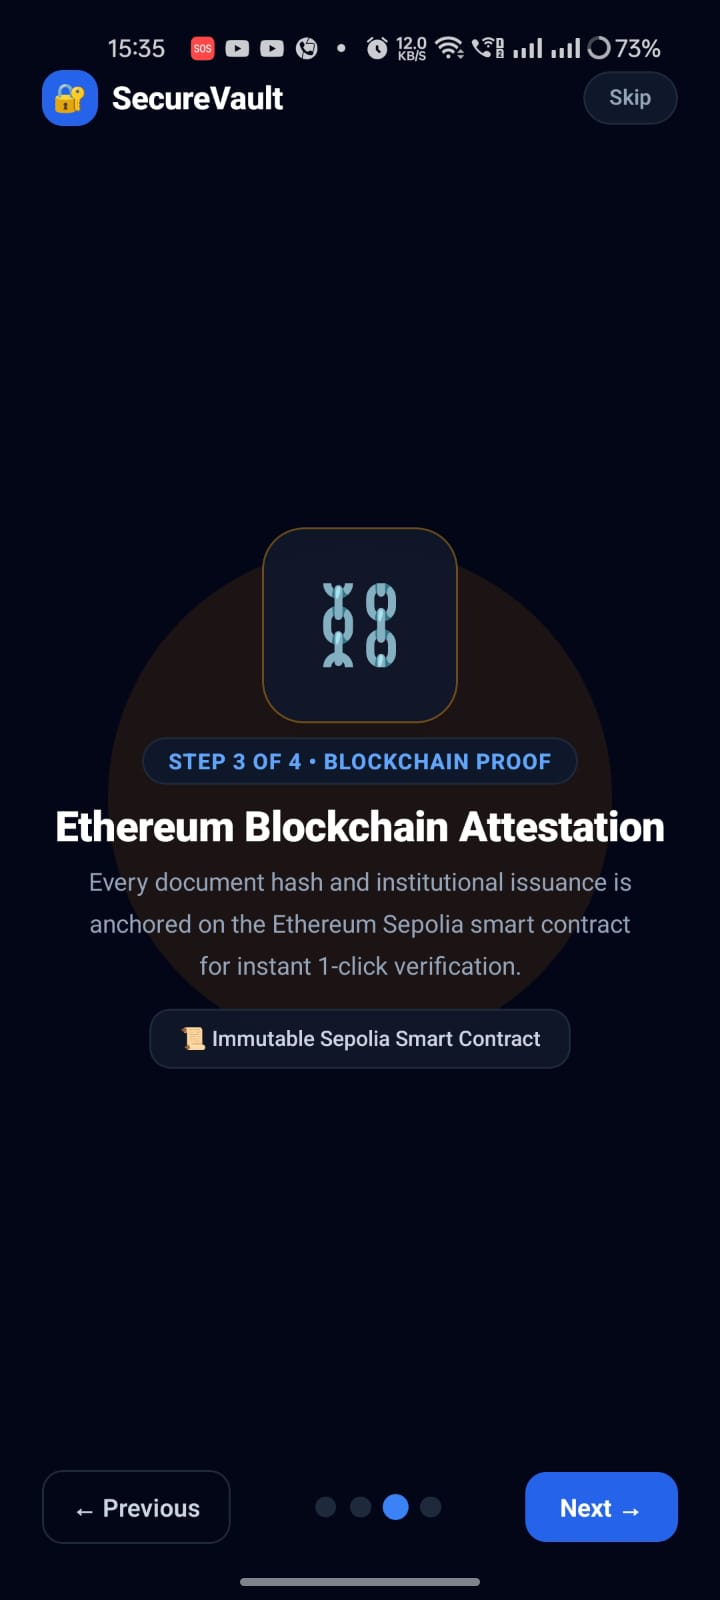
\includegraphics[width=6.5cm,height=9cm,keepaspectratio]{home3.jpeg}
    \caption{Secure Document Vault Home Page -- View 3}
    \label{fig:home-3}
\end{figure}

% Home Page - View 4
\begin{figure}[H]
    \centering
    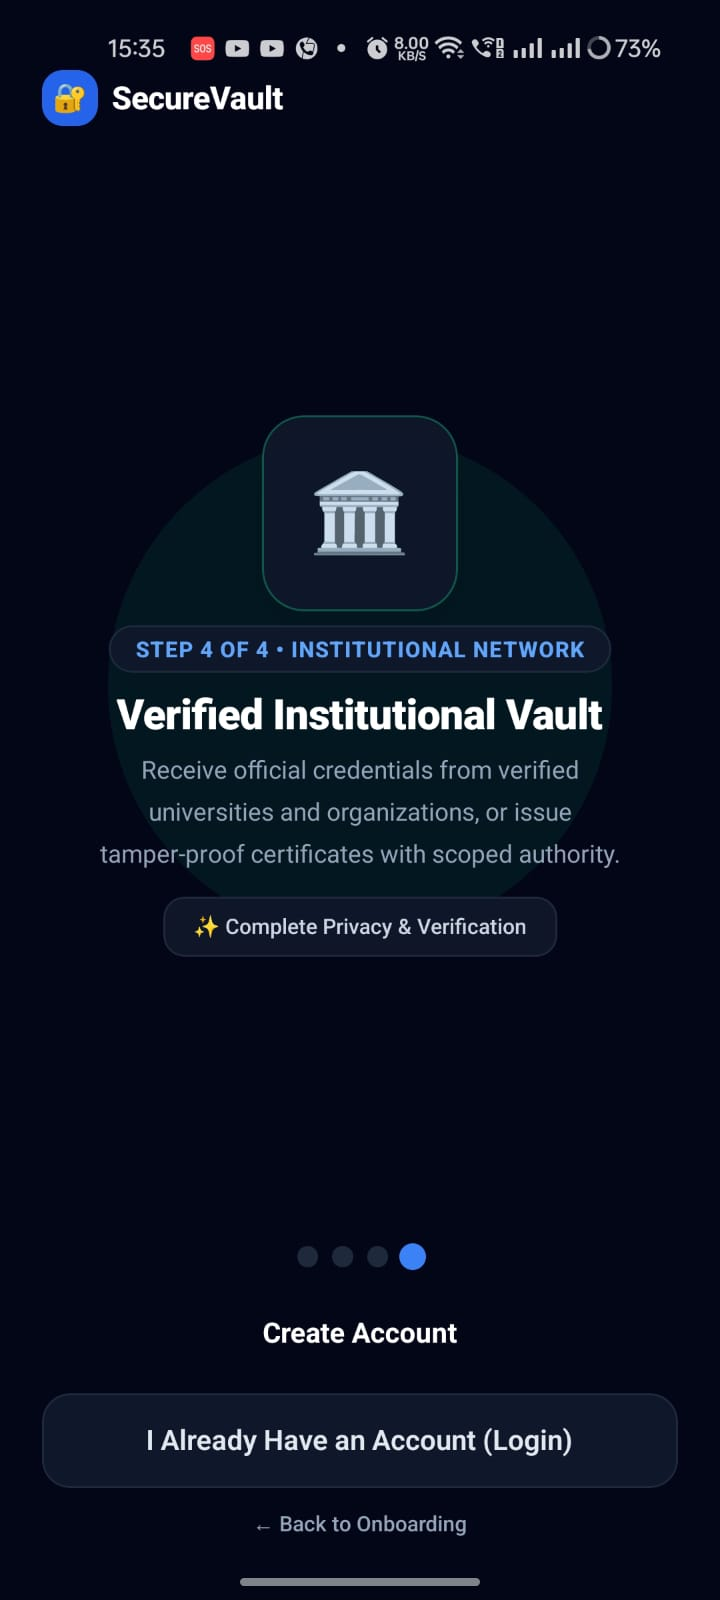
\includegraphics[width=6.5cm,height=9cm,keepaspectratio]{home4.jpeg}
    \caption{Secure Document Vault Home Page -- View 4}
    \label{fig:home-4}
\end{figure}

% User Registration using Email and Password
\begin{figure}[H]
    \centering
    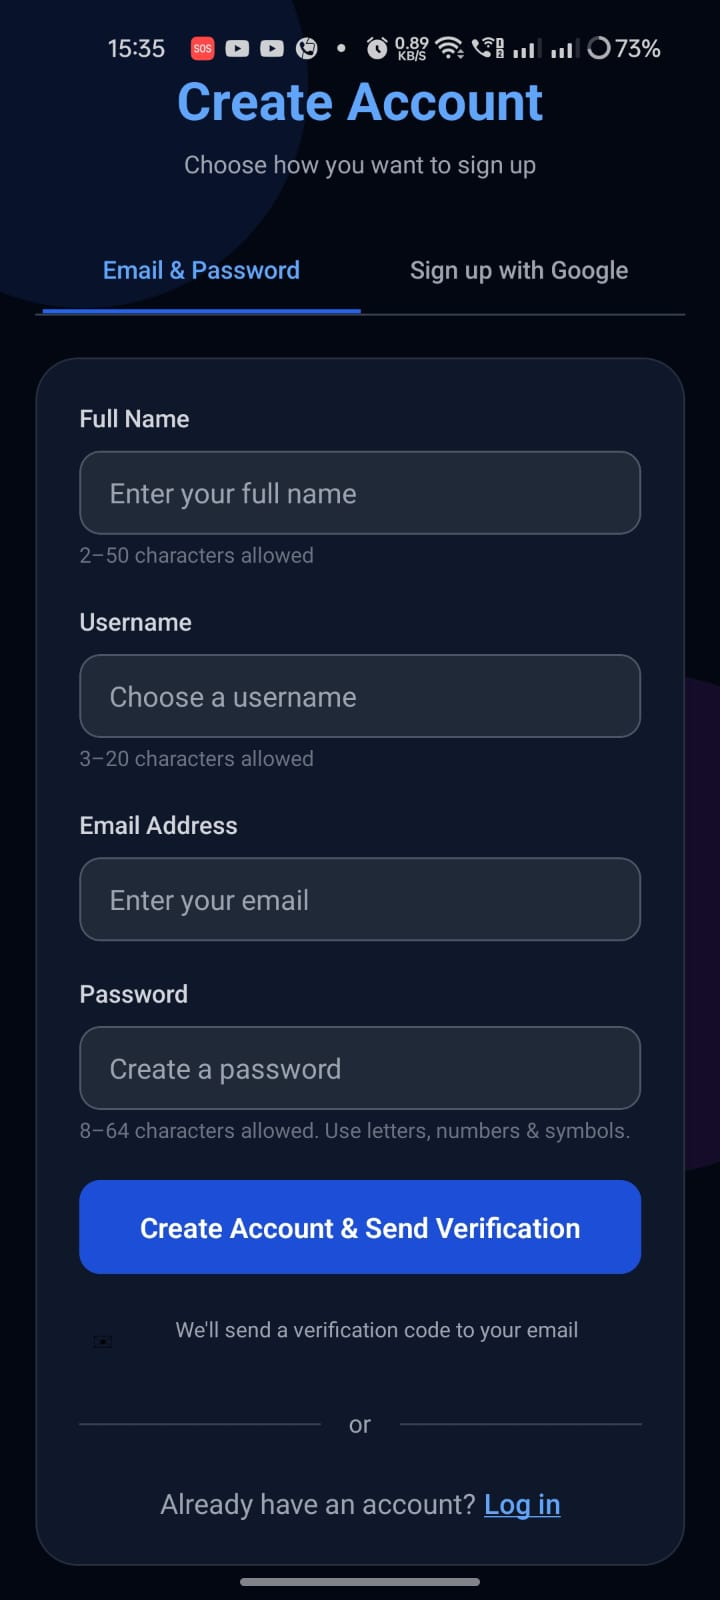
\includegraphics[width=6.5cm,height=9cm,keepaspectratio]{signupPassword.jpeg}
    \caption{User Registration Using Email and Password}
    \label{fig:signup-password}
\end{figure}

% User Registration using Google
\begin{figure}[H]
    \centering
    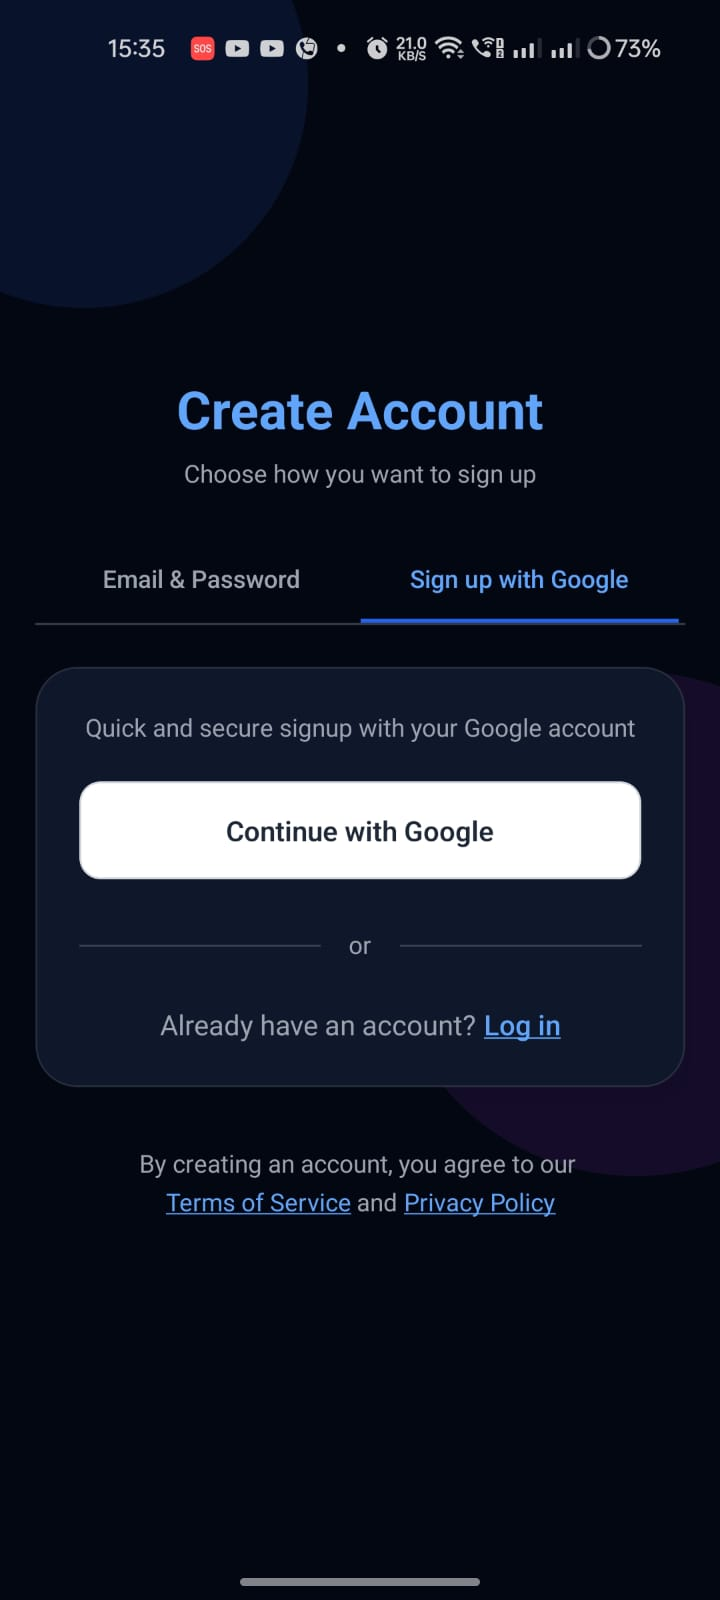
\includegraphics[width=6.5cm,height=9cm,keepaspectratio]{signupGoogle.jpeg}
    \caption{User Registration Using Google Authentication}
    \label{fig:signup-google}
\end{figure}

% User Sign In using Email and Password
\begin{figure}[H]
    \centering
    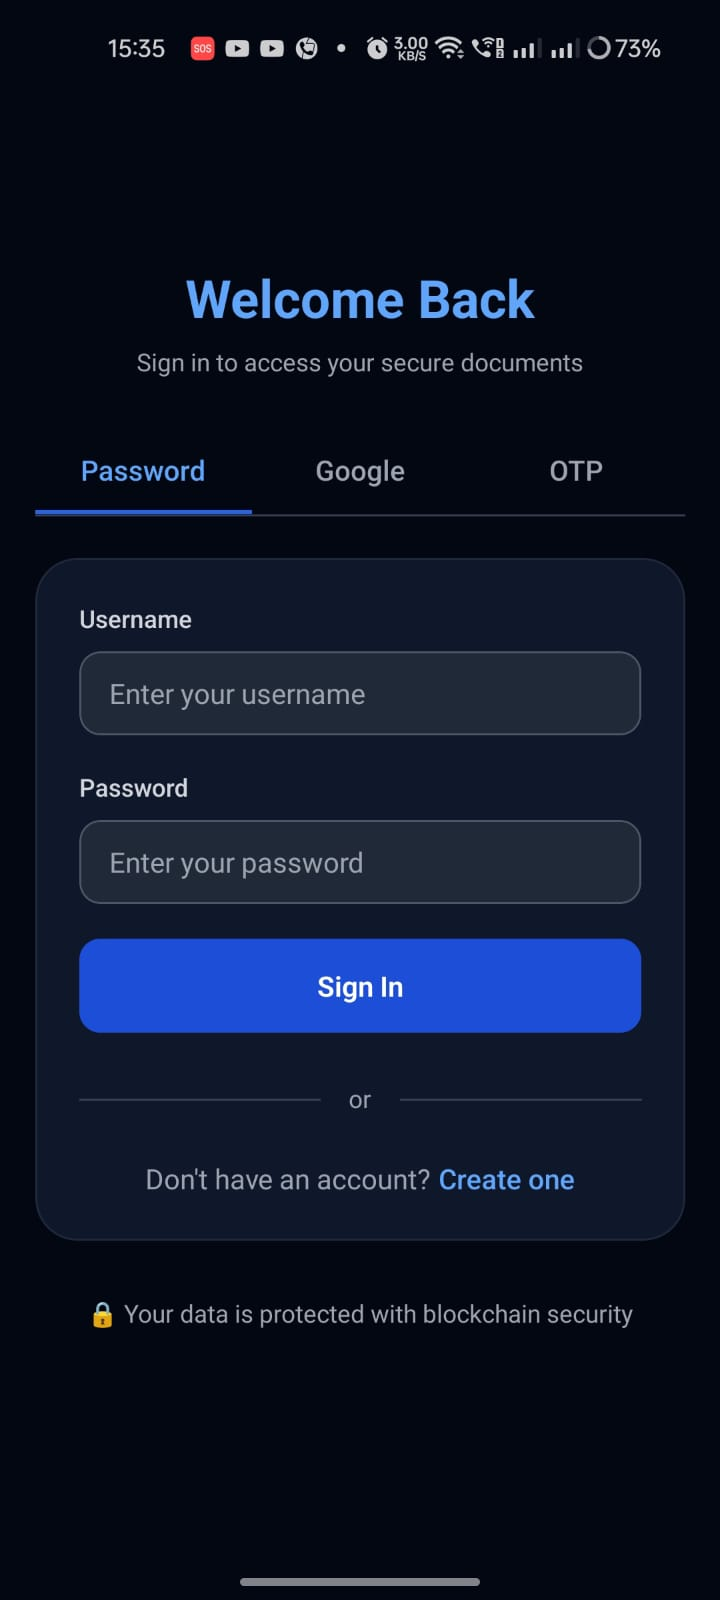
\includegraphics[width=6.5cm,height=9cm,keepaspectratio]{signinPassword.jpeg}
    \caption{User Sign In Using Email and Password}
    \label{fig:signin-password}
\end{figure}

% User Sign Up using OTP
\begin{figure}[H]
    \centering
    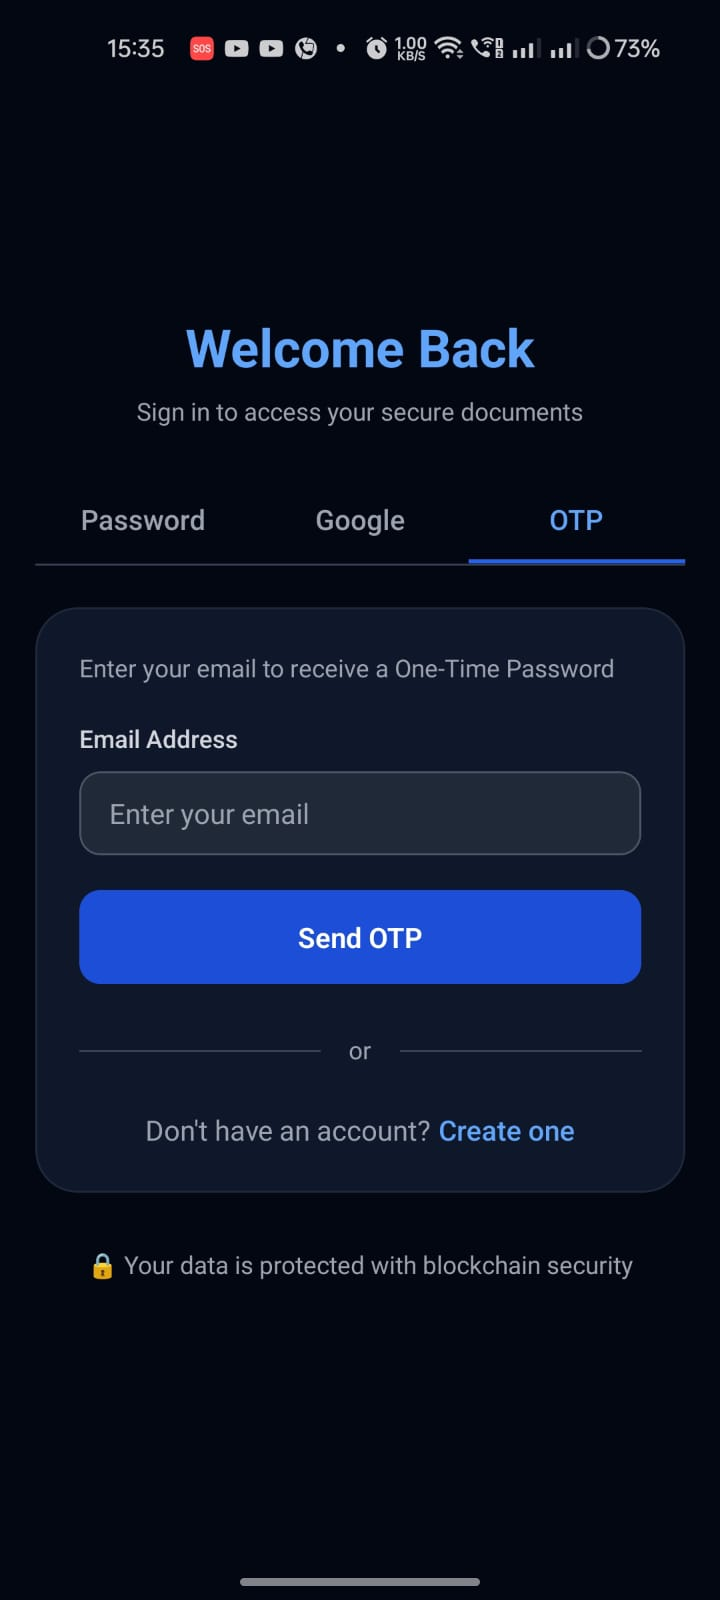
\includegraphics[width=6.5cm,height=9cm,keepaspectratio]{signOtp.jpeg}
    \caption{User Registration Using OTP Verification}
    \label{fig:signup-otp}
\end{figure}

% User Sign In using Google
\begin{figure}[H]
    \centering
    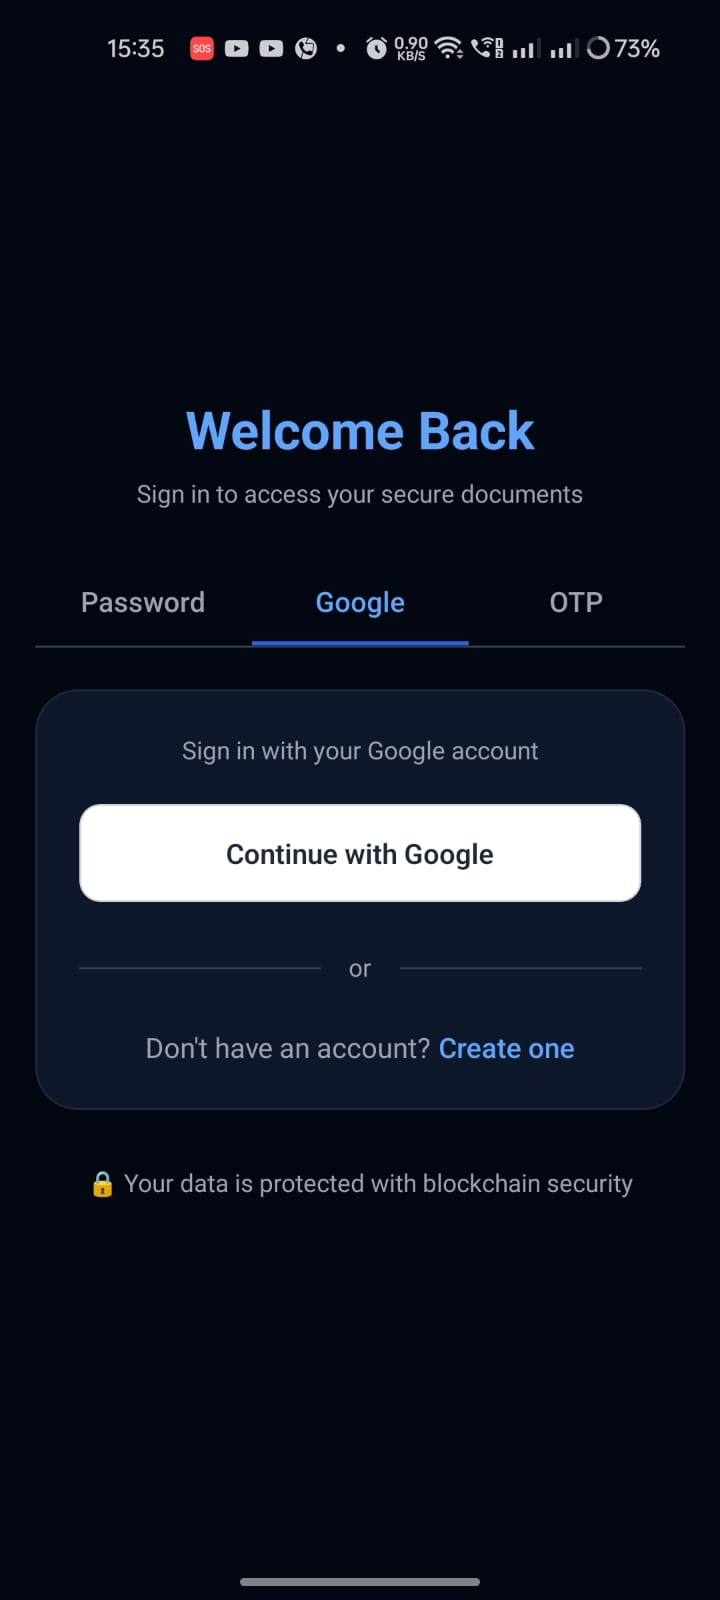
\includegraphics[width=6.5cm,height=9cm,keepaspectratio]{signinGoogle.jpeg}
    \caption{User Sign In Using Google Authentication}
    \label{fig:signin-google}
\end{figure}

% Home Page after Login
\begin{figure}[H]
    \centering
    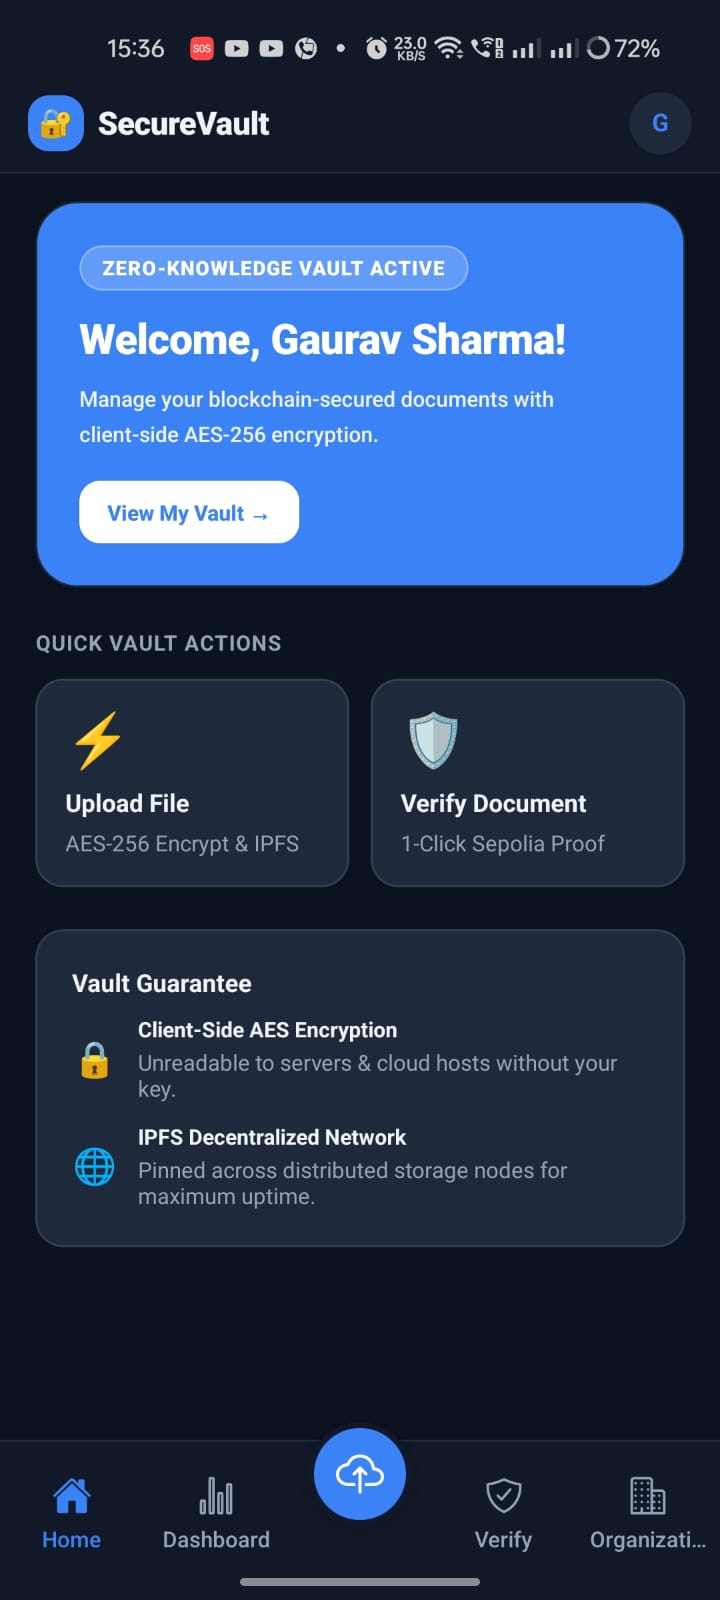
\includegraphics[width=6.5cm,height=9cm,keepaspectratio]{homeafter.jpeg}
    \caption{Secure Document Vault Home Page After User Authentication}
    \label{fig:home-after-login}
\end{figure}

% Dashboard
\begin{figure}[H]
    \centering
    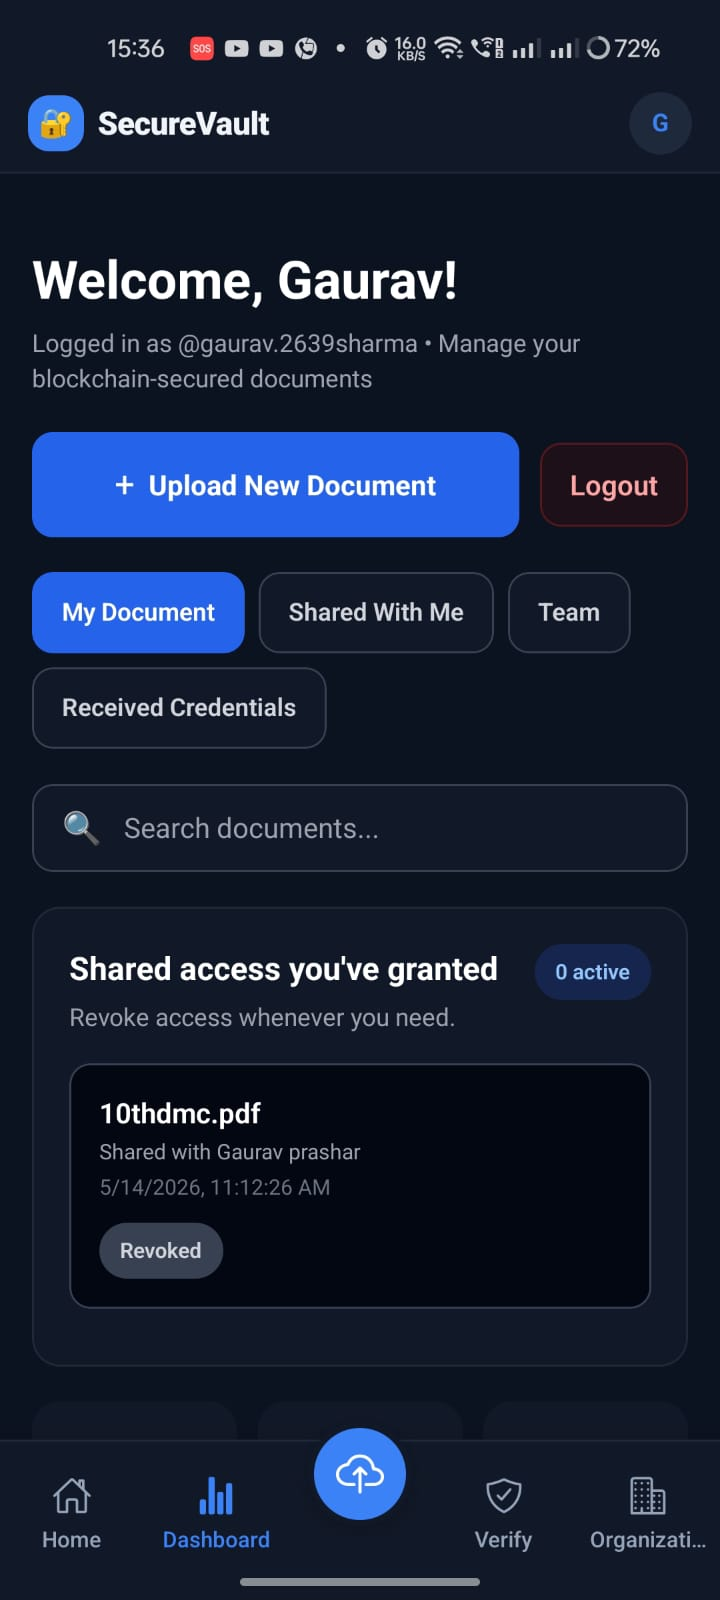
\includegraphics[width=6.5cm,height=9cm,keepaspectratio]{dashboard.jpeg}
    \caption{Secure Document Vault Dashboard}
    \label{fig:dashboard}
\end{figure}

% Document Upload
\begin{figure}[H]
    \centering
    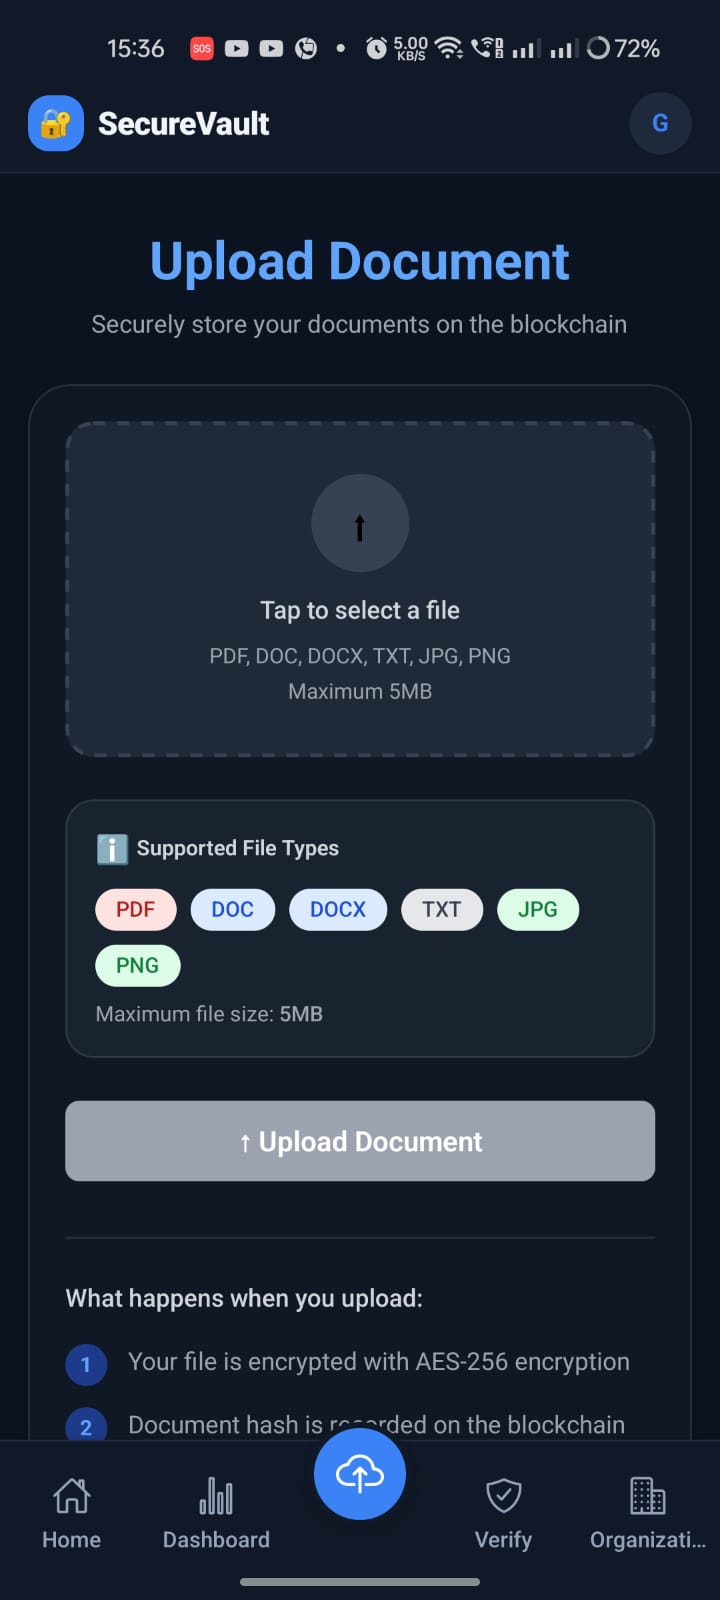
\includegraphics[width=6.5cm,height=9cm,keepaspectratio]{upload.jpeg}
    \caption{Document Upload Interface}
    \label{fig:upload}
\end{figure}

% Document Verification
\begin{figure}[H]
    \centering
    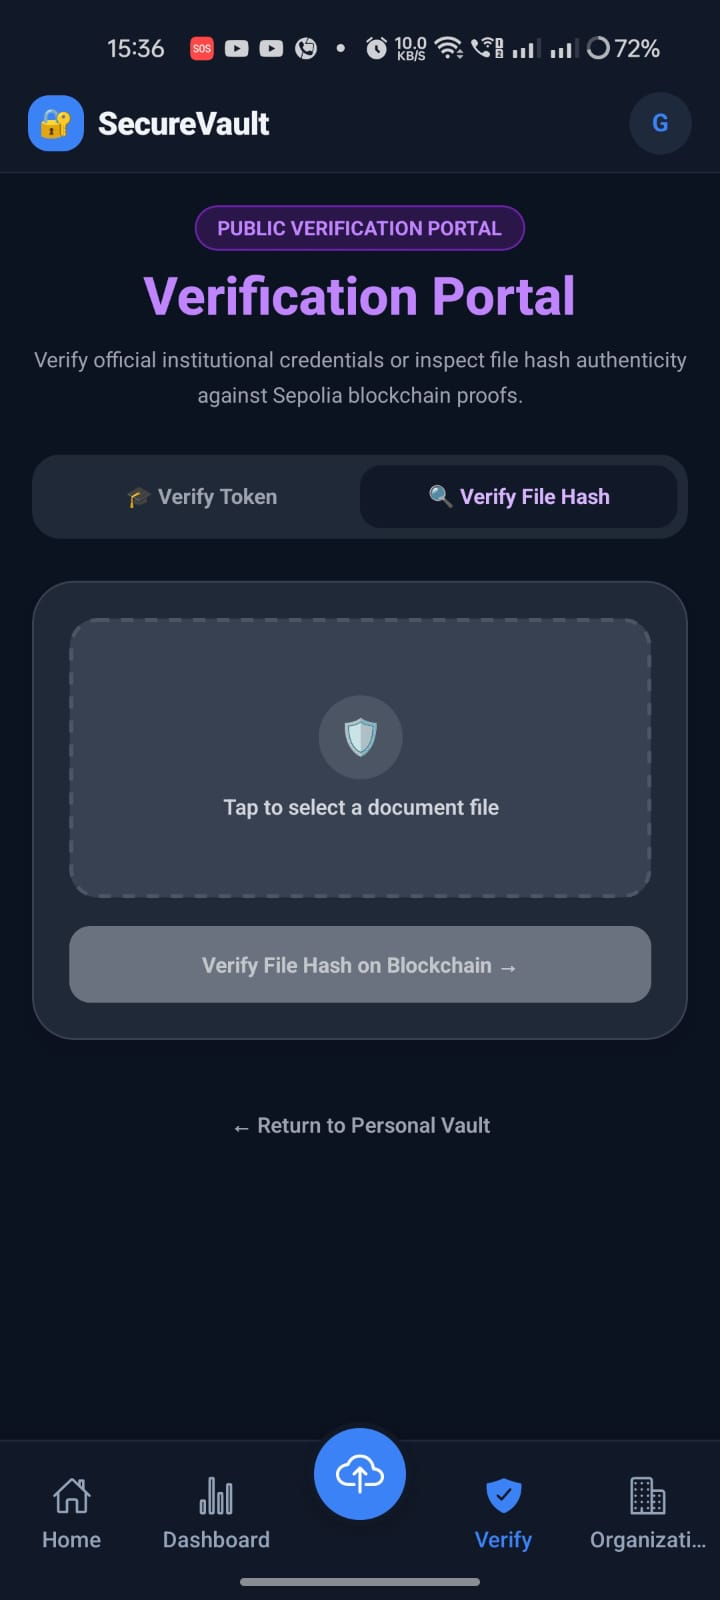
\includegraphics[width=6.5cm,height=9cm,keepaspectratio]{verify.jpeg}
    \caption{Document Verification Interface}
    \label{fig:verification}
\end{figure}

% Organization Dashboard
\begin{figure}[H]
    \centering
    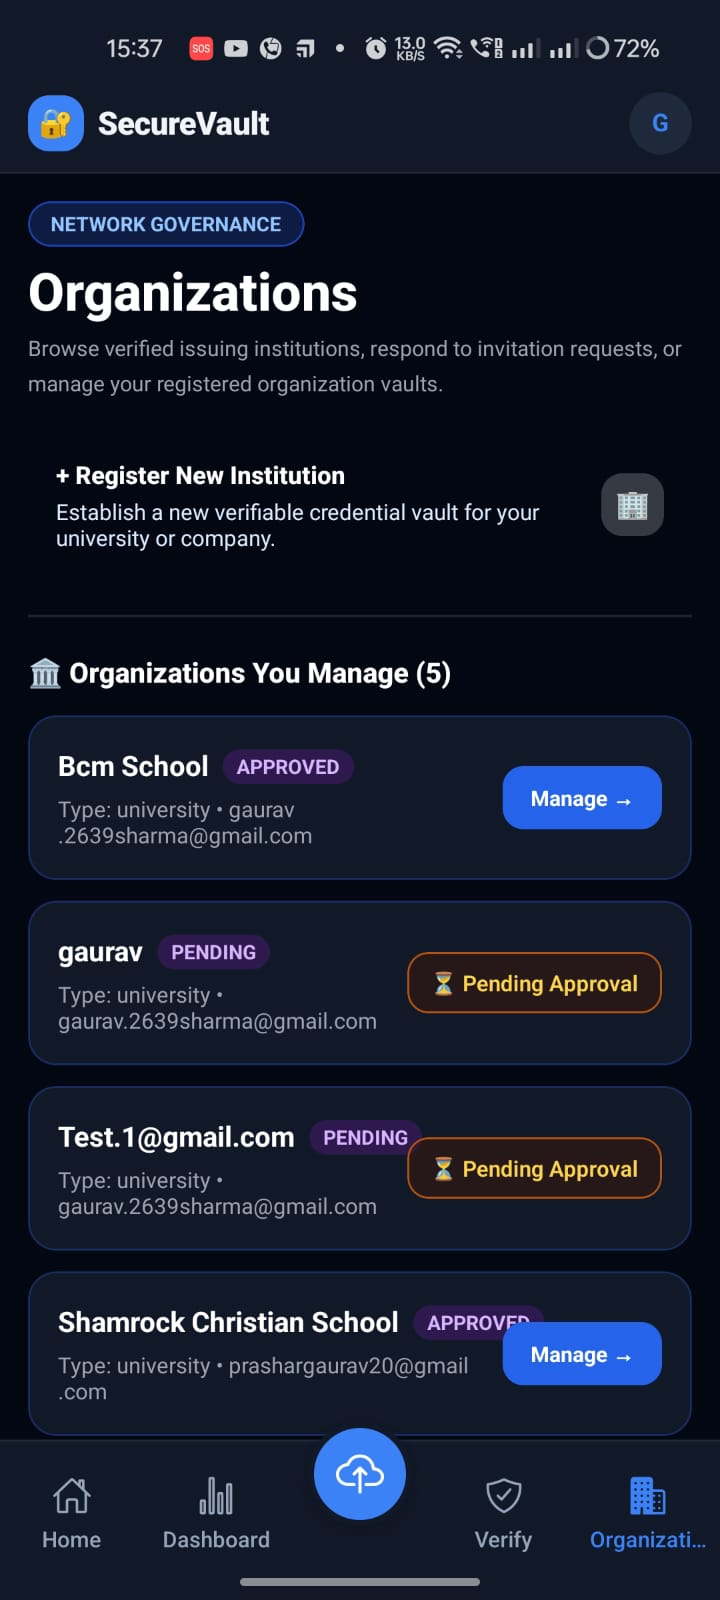
\includegraphics[width=6.5cm,height=9cm,keepaspectratio]{organization.jpeg}
    \caption{Organization Dashboard}
    \label{fig:organization-dashboard}
\end{figure}

% Organization Registration
\begin{figure}[H]
    \centering
    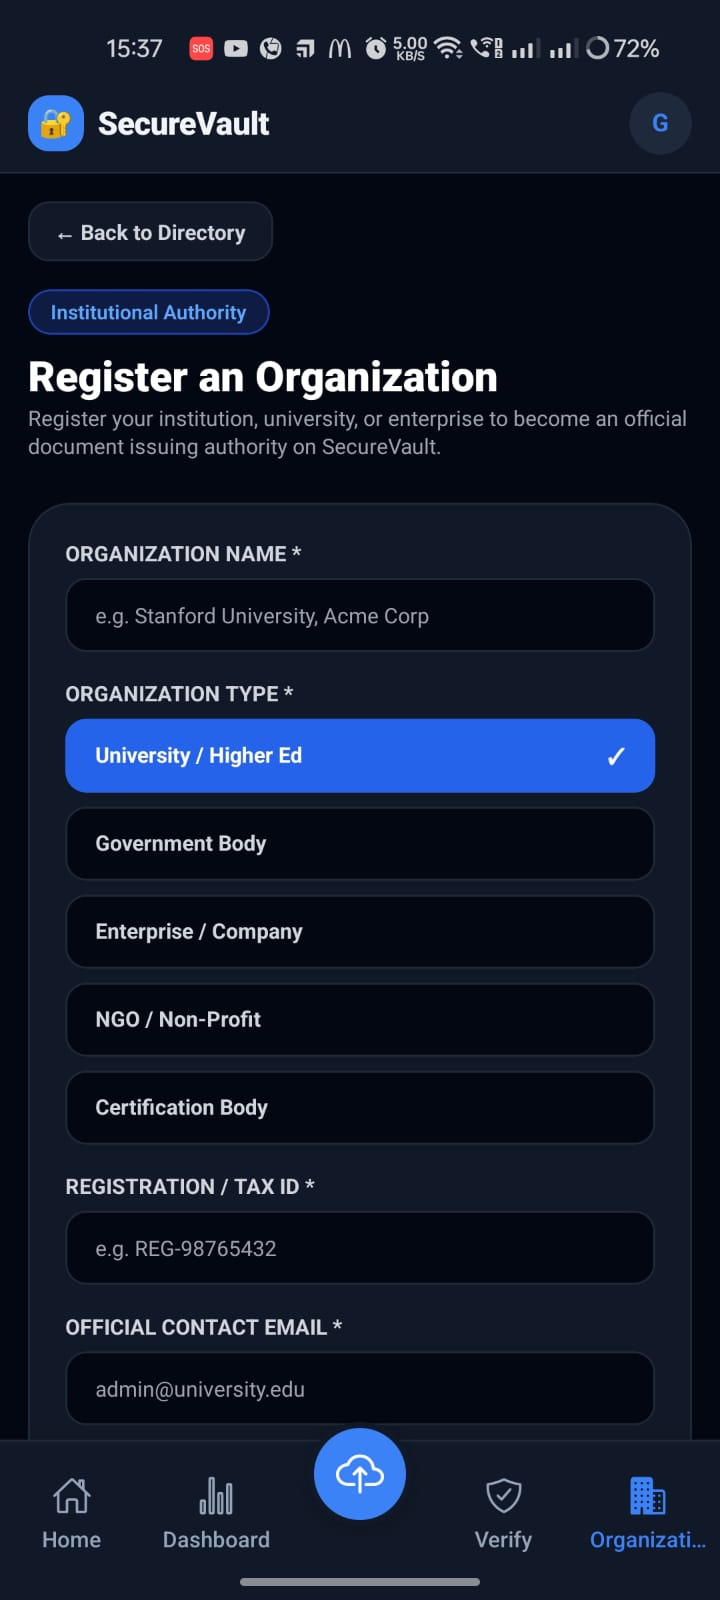
\includegraphics[width=6.5cm,height=9cm,keepaspectratio]{oganizationRegister.jpeg}
    \caption{Organization Registration Interface}
    \label{fig:organization-registration}
\end{figure}

% Organization Management
\begin{figure}[H]
    \centering
    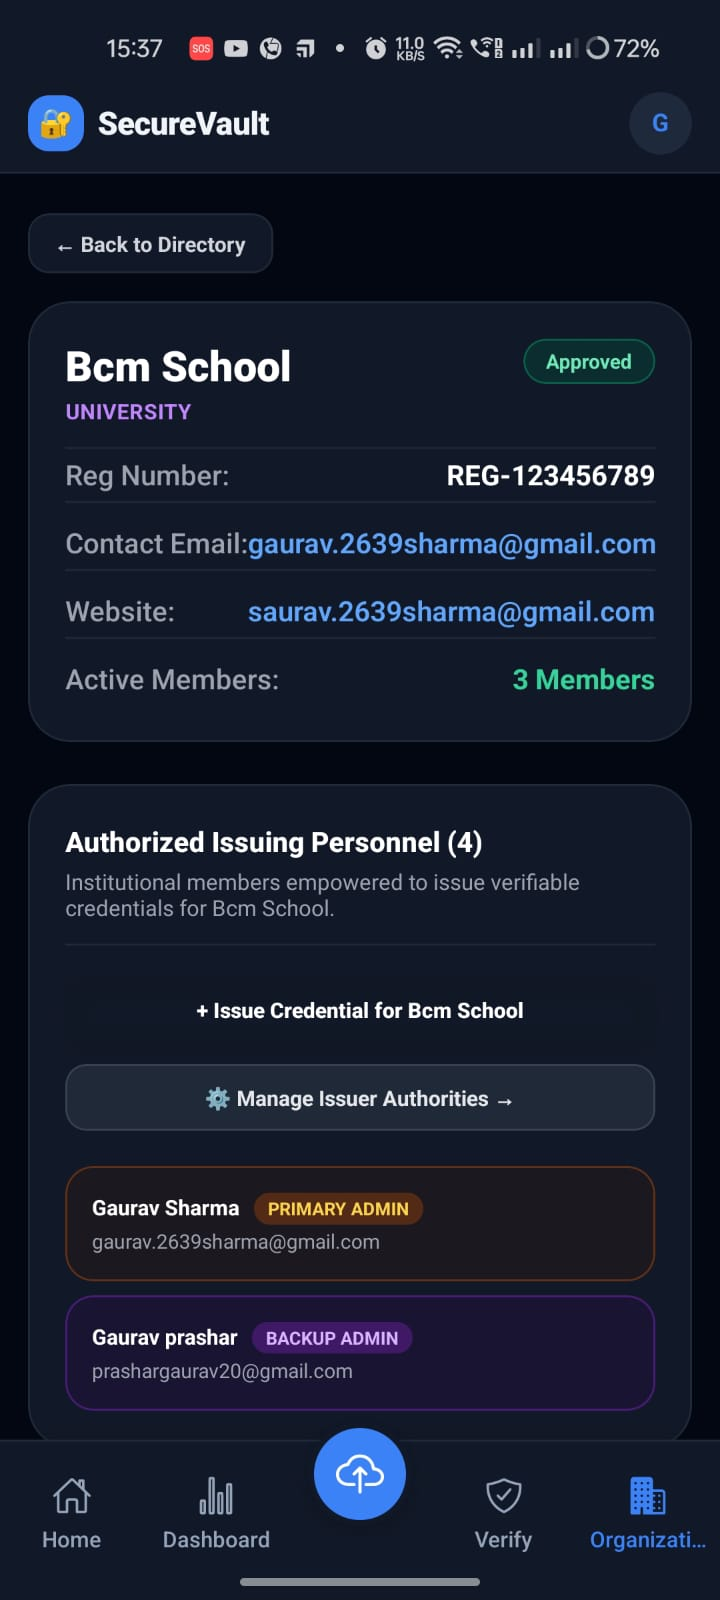
\includegraphics[width=6.5cm,height=9cm,keepaspectratio]{organizationManagement.jpeg}
    \caption{Organization Management Interface}
    \label{fig:organization-management}
\end{figure}

% Profile and Logout
\begin{figure}[H]
    \centering
    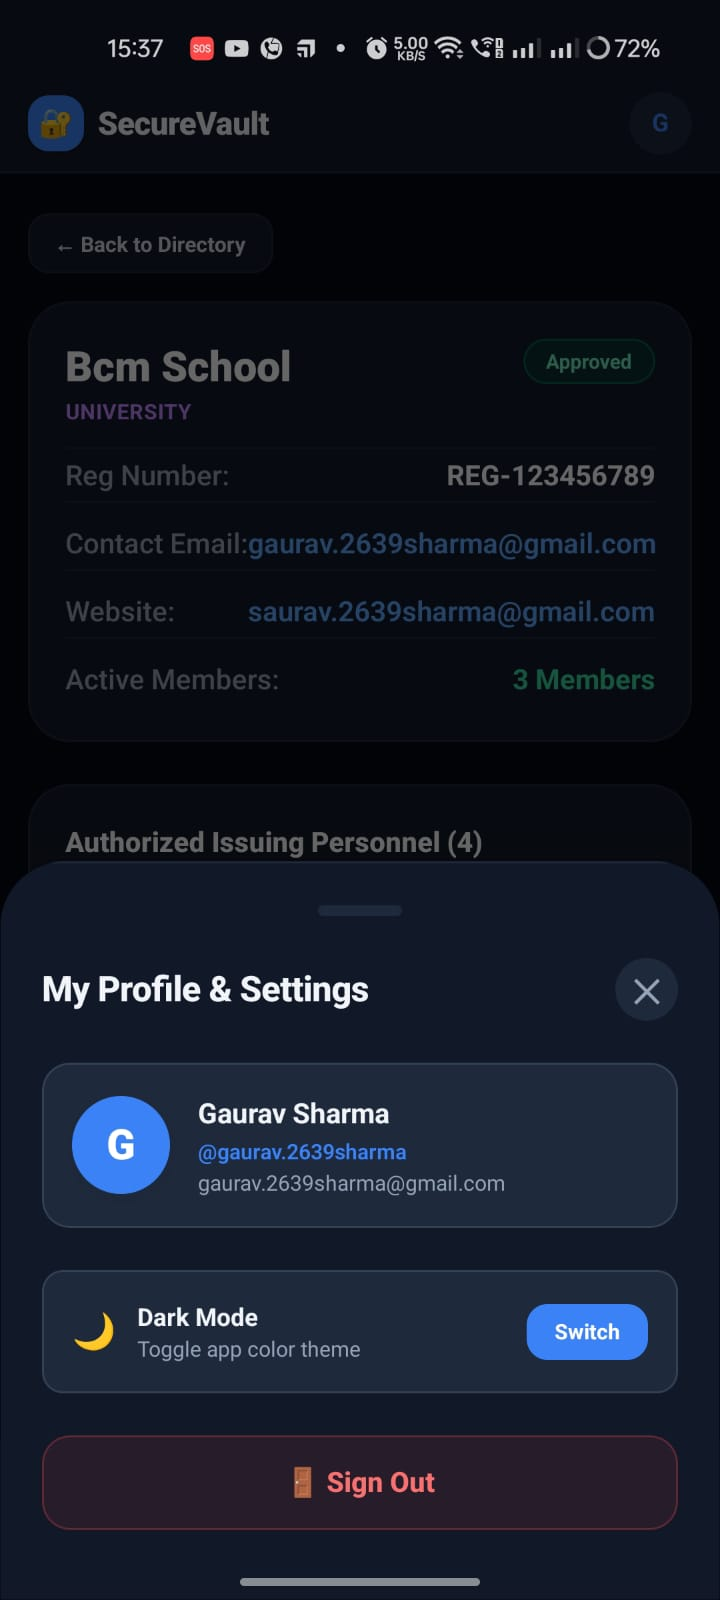
\includegraphics[width=6.5cm,height=9cm,keepaspectratio]{logout.jpeg}
    \caption{User Profile Information and Logout Interface}
    \label{fig:profile-logout}
\end{figure}

\newpage
\bibliographystyle{IEEEtran}
\bibliography{references}

\end{document}
